% Created 2022-06-07 Tue 18:38
% Intended LaTeX compiler: pdflatex
\documentclass[twoside, twocolumn, 9pt, draft]{article}
\usepackage[utf8]{inputenc}
\usepackage[T1]{fontenc}
\usepackage{graphicx}
\usepackage{longtable}
\usepackage{wrapfig}
\usepackage{rotating}
\usepackage[normalem]{ulem}
\usepackage{amsmath}
\usepackage{amssymb}
\usepackage{capt-of}
\usepackage{hyperref}
\usepackage[acronym,nogroupskip,nonumberlist]{glossaries}
\usepackage[%
stylemods,style=long-short,
]{glossaries-extra}
\makeglossaries
\usepackage{abstract}%% easy abstract environment (from frontmatter pkg "ltxfront")
\usepackage[export]{adjustbox}%% expanded control over image, minipages, etc
\usepackage{sectsty}%% control of section heading appearance in default and script doc classes
\usepackage{setspace}%% implements \setstretch for line spacing
\usepackage{amsthm}%% formal mathematics environments
\usepackage{mathtools}%% bugfixing and additional tools for amsmath
\usepackage{lastpage}%% allows ref to lastpage
\usepackage{amsfonts}%% formal math fonts
\usepackage{mathptmx}%% ghostscript/postscript fonts and font loading options
\usepackage{charter}%% ghostscript/postscript fonts outside of math envs
\usepackage{times}%% more ghostscript/postscript
\usepackage{bm}%% bold math
\usepackage[%% full (expands on capt-of) control over appearance of float captions
%margin=10pt
format=plain,
justification=justified,
singlelinecheck=false,
font={small, sf},
labelfont=bf,
labelsep=space
]{caption}%% global preamble, use \captionsetup{} to config env)

\usepackage[compact]{titlesec}%% replacement of sectioning macros, coexsiting with old stuff
\usepackage{fancyhdr}%% improved headers and footers
\usepackage{fnpos}%% footnote positioning tools
\usepackage{sidecap}%% control of figure and caption positioning and margin spill
\usepackage{gensymb}%% inter-environment consistent measurment unit symbols
\usepackage{upgreek}%% easy lower and uppercase nonitalicized greek letters
\usepackage{soul}%% spaceout and underline macros

\usepackage{array}%% modernization of array and tabular envs
\usepackage{droidsans}%% use android sanserif fonts...

\usepackage[usenames,dvipsnames]{xcolor}%% text color macros
\usepackage[version=3]{mhchem}%% for writing chemical formulae
\usepackage[super,sort&compress,comma]{natbib}%% prefered citation engine

%% control margin configurations and visualize framing
\usepackage[%%rsc page standard follows
left=1.5cm,
right=1.5cm,
top=1.785cm,
bottom=2.0cm
]{geometry}

\addto{\captionsenglish}{%
\renewcommand{\refname}{Notes and references}
}

\definecolor{cream}{RGB}{222,217,201}%% required for use of rsc frontmatter

%\usepackage[mathlines]{lineno}%% Enable numbering of text and display math
%\linenumbers\relax%% Commence numbering lines
\newglossaryentry{vasp}{name=VASP,description={{Vienna Ab initio Simulation Package}}}
\newglossaryentry{slme}{name=SLME,description={{Spectroscopic Limited Maximum Efficiency}}}
\newglossaryentry{qmml}{name=QM/ML,description={{Quantum Mechanics Machine Learning}}}
\newglossaryentry{pca}{name=PCA,description={{Principal Component Analysis}}}
\newglossaryentry{tsne}{name=t-SNE,description={{t-distributed Stochastic Neighbor Embedding}}}
\newglossaryentry{umap}{name=UMAP,description={{Uniform Manifold Approximation and Projection}}}
\newacronym{dft}{DFT}{Density Functional Theory}
\newacronym{sqs}{SQS}{special quasi-random structures}
\newacronym{paw}{PAW}{projector augmented wave}
\newacronym{gga}{GGA}{generalized gradient approximation}
\newacronym{pbe}{PBE}{Perdew-Burke-Ernzerhof}
\newacronym{hse}{HSE}{Heyd-Scuseria-Ernzerhof}
\newacronym{ma}{MA}{Methylammonium}
\newacronym{fa}{FA}{Formamidinium}
\newacronym{pce}{PCE}{Power Conversion Efficiency}
\date{\today}
\title{A High-Throughput Computational Dataset of Halide Perovskite Alloys\textsuperscript{\dag}}
\hypersetup{
 pdfauthor={Panayotis Manganaris},
 pdftitle={A High-Throughput Computational Dataset of Halide Perovskite Alloys\textsuperscript{\dag}},
 pdfkeywords={},
 pdfsubject={},
 pdfcreator={Emacs 29.0.50 (Org mode 9.5.3)}, 
 pdflang={English}}
\begin{document}

% Royal Society of Chemistry frontmatter conventions for quick recall via INCLUDE keyword

\pagestyle{fancy}
\thispagestyle{plain}
\fancypagestyle{plain}{
%%%HEADER%%%
\renewcommand{\headrulewidth}{0pt}
}
%%%END OF HEADER%%%

%%%PAGE SETUP - Please do not change any commands within this section%%%
\makeFNbottom
\makeatletter
\renewcommand\LARGE{\@setfontsize\LARGE{15pt}{17}}
\renewcommand\Large{\@setfontsize\Large{12pt}{14}}
\renewcommand\large{\@setfontsize\large{10pt}{12}}
\renewcommand\footnotesize{\@setfontsize\footnotesize{7pt}{10}}
\makeatother

\renewcommand{\thefootnote}{\fnsymbol{footnote}}
\renewcommand\footnoterule{\vspace*{1pt}% 
\color{cream}\hrule width 3.5in height 0.4pt \color{black}\vspace*{5pt}} 
\setcounter{secnumdepth}{5}

\makeatletter 
\renewcommand\@biblabel[1]{#1}            
\renewcommand\@makefntext[1]{\noindent\makebox[0pt][r]{\@thefnmark\,}#1}
\makeatother 
\renewcommand{\figurename}{\small{Fig.}~}
\sectionfont{\sffamily\Large}
\subsectionfont{\normalsize}
\subsubsectionfont{\bf}
\setstretch{1.125}
\setlength{\skip\footins}{0.8cm}
\setlength{\footnotesep}{0.25cm}
\setlength{\jot}{10pt}
\titlespacing*{\section}{0pt}{4pt}{4pt}
\titlespacing*{\subsection}{0pt}{15pt}{1pt}
%%%END OF PAGE SETUP%%%

%%%FOOTER%%%
\fancyfoot{}
\fancyfoot[LO,RE]{\vspace{-7.1pt}\includegraphics[height=9pt]{head_foot/LF}}
\fancyfoot[CO]{\vspace{-7.1pt}\hspace{13.2cm}\includegraphics{head_foot/RF}}
\fancyfoot[CE]{\vspace{-7.2pt}\hspace{-14.2cm}\includegraphics{head_foot/RF}}
\fancyfoot[RO]{\footnotesize{\sffamily{1--\pageref{LastPage} ~\textbar  \hspace{2pt}\thepage}}}
\fancyfoot[LE]{\footnotesize{\sffamily{\thepage~\textbar\hspace{3.45cm} 1--\pageref{LastPage}}}}
\fancyhead{}
\renewcommand{\headrulewidth}{0pt} 
\renewcommand{\footrulewidth}{0pt}
\setlength{\arrayrulewidth}{1pt}
\setlength{\columnsep}{6.5mm}
\setlength\bibsep{1pt}
%%%END OF FOOTER%%%

%%%FIGURE SETUP - please do not change any commands within this section%%%
\makeatletter 
\newlength{\figrulesep} 
\setlength{\figrulesep}{0.5\textfloatsep} 

\newcommand{\topfigrule}{\vspace*{-1pt}% 
\noindent{\color{cream}\rule[-\figrulesep]{\columnwidth}{1.5pt}} }

\newcommand{\botfigrule}{\vspace*{-2pt}% 
\noindent{\color{cream}\rule[\figrulesep]{\columnwidth}{1.5pt}} }

\newcommand{\dblfigrule}{\vspace*{-1pt}% 
\noindent{\color{cream}\rule[-\figrulesep]{\textwidth}{1.5pt}} }

\makeatother
%%%END OF FIGURE SETUP%%%

%%%TITLE, AUTHORS AND ABSTRACT%%%
\twocolumn[
\begin{@twocolumnfalse}
{%\includegraphics[height=30pt]{head_foot/journal_name}\hfill\raisebox{0pt}[0pt][0pt]{\includegraphics[height=55pt]{head_foot/RSC_LOGO_CMYK}}\\[1ex]
%\includegraphics[width=18.5cm]{head_foot/header_bar}}\par
\vspace{1em}
\sffamily
\begin{tabular}{m{4.5cm} p{13.5cm} }
%\includegraphics{head_foot/DOI}
& \noindent\LARGE{\textbf{A High-Throughput Computational Dataset of Halide Perovskite Alloys\textsuperscript{\dag}}}\\%
%Article title goes here
\vspace{0.3cm} & \vspace{0.3cm} \\
& \noindent\large{Jiaqi Yang\textsuperscript{a}, Panayotis Manganaris\textsuperscript{a}, and Arun Mannodi-Kanakkithodi\textsuperscript{a}}}\\
%Author names go here
\end{tabular}
\begin{abstract}
Novel halide Perovskites with improved stability and optoelectronic properties can be designed via composition engineering at cation and/or
anion sites. Data-driven methods, especially high-throughput first principles computations and subsequent analysis based on unique materials
descriptors, are key to achieving this goal. In this work, we report a Density Functional Theory (DFT) based dataset of 495 ABX\textsubscript{3} halide
Perovskite compounds, with various atomic and molecular species considered at A, B and X sites, and different amounts of mixing considered
at each site generated using the Special Quasirandom Structures (SQS) algorithm for alloys. We perform GGA-PBE calculations on pseudo-cubic
Perovskite structures to determine their lattice constants, stability in terms of formation and decomposition energies, electronic band gaps,
and properties extracted from optical absorption spectra. To elucidate the importance of the level of theory used, we further perform 299 calculations
using the more expensive HSE06 functional and determine lattice constant, stability and band gap, and compare PBE and HSE06 properties with
some experimentally measured results. Trends in the datasets are unraveled in terms of the effects of mixing at different sites, the
composition in terms of specific atomic or molecular species, and averaged elemental properties of species at different sites. This work
presents the most comprehensive DFT perovskite alloy dataset to date and the data, which is open-source, can be exploited to train
predictive and optimization models for accelerating the design of completely new compositions that may yield large solar cell efficiencies
and improved performance across many optoelectronic applications.
\end{abstract}
\end{@twocolumnfalse}
\vspace{0.6cm}
]
%%%END OF TITLE, AUTHORS AND ABSTRACT%%%

%%%FONT SETUP - please do not change any commands within this section
\renewcommand*\rmdefault{bch}\normalfont\upshape
\rmfamily
\section*{}
\vspace{-1cm}

%INCLUDE -- notice abstract is contained in titleblock

\footnotetext{\textsuperscript{a}School of Materials Engineering, Purdue University, West Lafayette, IN 47907, USA; E-mail: amannodi@purdue.edu}
\footnotetext{\textsuperscript{\dag}Electronic Supplementary Information (ESI) available: https://www.github.com/PanayotisManganaris/REPO_TODO. See DOI: 00.0000/00000000.}

\section*{{\bfseries\sffamily TODO} Introduction}
\label{sec:orgb26b3ec}
\begin{itemize}
\item State "DONE"       from              \textit{[2022-06-05 Sun 18:16]}
\end{itemize}
The challenge of optimizing Perovskite performance is one with many
facets. Almost every detail of a Perovskite crystal's structure and
chemistry effects its performance as a semiconductor. The size of the
unit cell effects its substrate affinity and in turn its carrier
concentrations \cite{jiang-2006-predic-lattic}. The crystal's phase
effects many aspects of the electronic structure, including the band
gap and optical response. Of course, these qualities of a structure
are largely dependent on the specification, proportions and
arrangements of the constituent elements.

We report a synthetic dataset collected for 495 chemically distinct,
pseudo cubic Halide Perovskites. This dataset builds on that of 229
samples which formed the foundation of the prior work by
\citet{mannodi-kanakkithodi-2021-data-driven-new}. The
\acrfull{dft} computed properties we collected and the levels
of theory used are discussed in \hyperref[sec:orgefce05d]{Methodology}. The relatively large
size of this dataset is intended to provide an initial sampling
suitable for guiding exploration of the alloy space. Structural
information is considered constant to better focus on obtaining
physically meaningful interpretations of models dealing only with
information derived from a sample composition.

literature review about grouping/unsupervised learning

\begin{figure*}
\centering
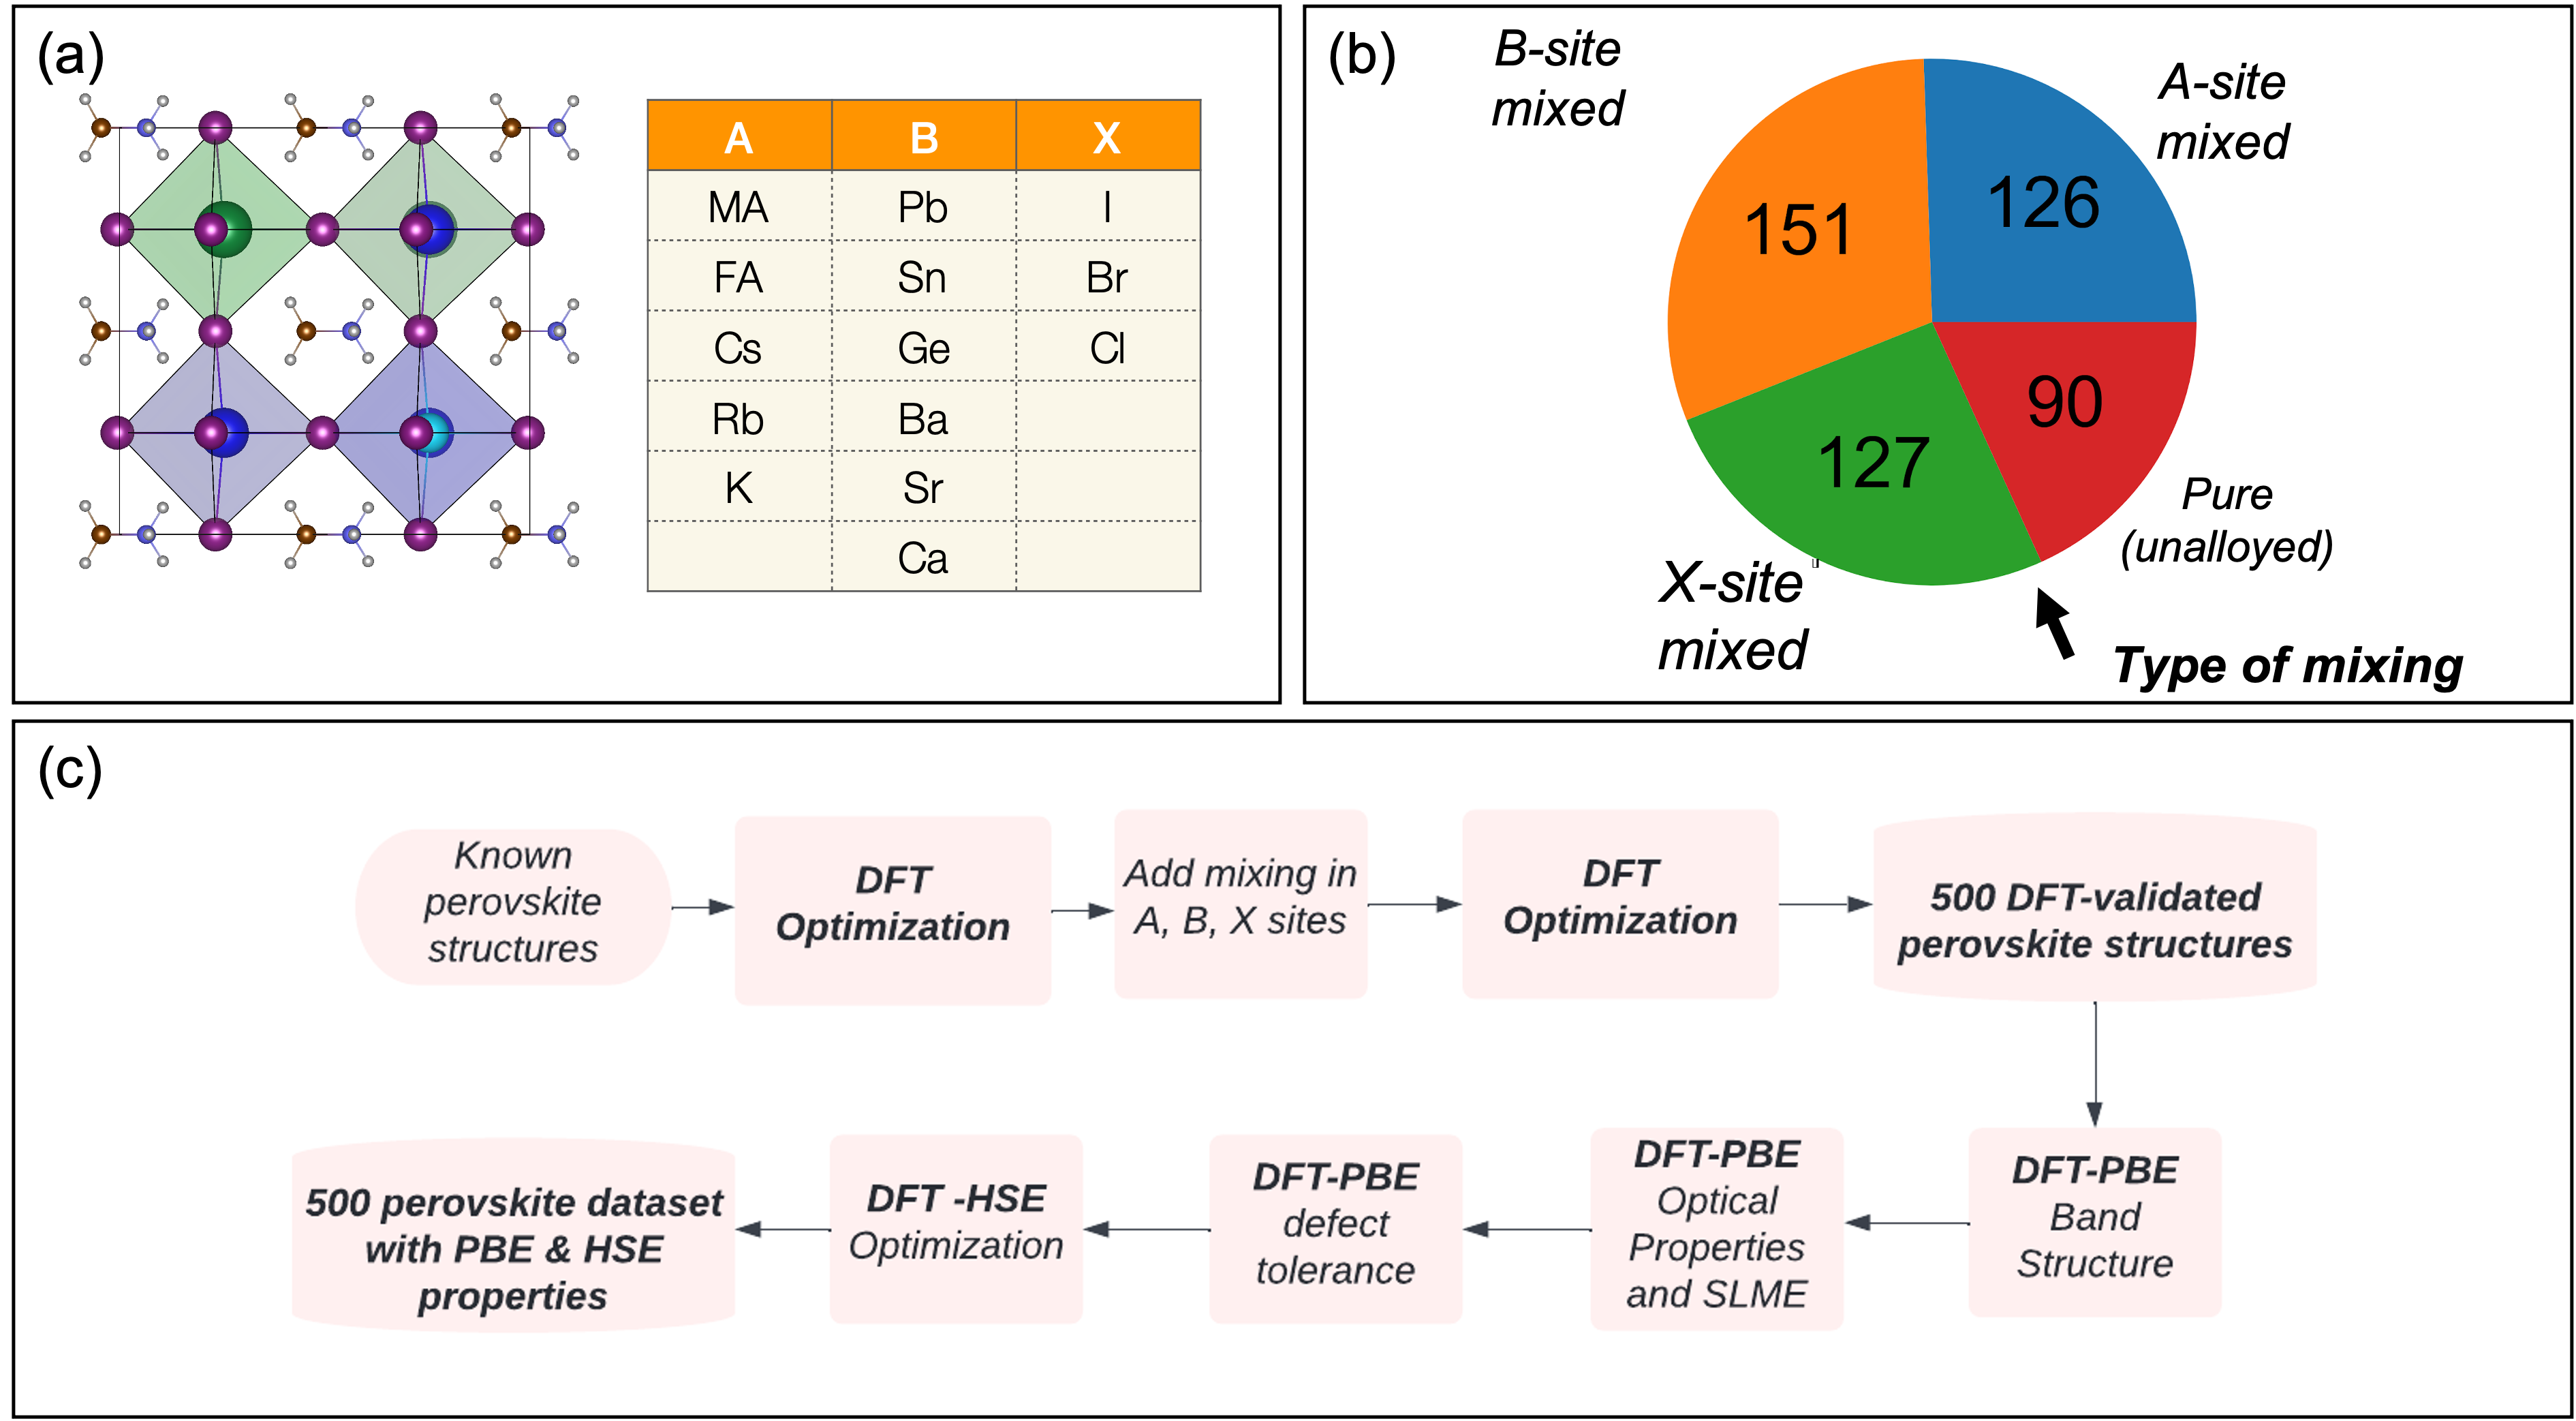
\includegraphics[h,width=.9\linewidth]{outline.png}
\caption{\label{fig:outline} (a) Chemical space of ABX\textsubscript{3} perovskites. (b) Number of samples representing each kind of primary alloy. (c) Detailed outline.}
\end{figure*}

\section*{{\bfseries\sffamily TODO} Methodology}
\label{sec:orgefce05d}
\subsection*{{\bfseries\sffamily NEXT} Building Perovskite Dataset}
\label{sec:org41fc490}
\begin{itemize}
\item State "NEXT"       from "TODO"       \textit{[2022-06-05 Sun 22:11]}
\end{itemize}
The dataset we report is based on standard cubic phase ABX\textsubscript{3}
Perovskite structures obtained from public databases. Fourteen common
Perovskite constituents are selected to form our Halide Perovskite
composition space (Figure \ref{fig:outline}). Five constituents
including \acrfull{ma} and \acrfull{fa} cations represent
the possible A-site occupants. Six metals represent the possible
B-site occupants. Three halides represent the possible X-site
occupants. In total, these component vectors form a constrained 14
dimensional space (Figure \ref{fig:chemspace_uni}) within which all
Perovskite compounds consisting of the elements in Figure
\ref{fig:outline} (a) must exist.

The pure (non-alloyed) possibilities are exhaustively sampled using
\(5*6*3 = 90\) Perovskites. Based on these pure Perovskite structures,
we mix candidates for A, B, and X sites systematically. The alloy
space sees combinatorial scaling and must be sparsely sampled (Figure
\ref{fig:sample_map}).

To generate site-mixing structures with high representativeness,
\acrfull{sqs} are applied. The \acrshort{sqs} method is
to build a special periodic structure and make the first
nearest-neighbor shells as similar to the target random alloy as
possible. The \acrshort{sqs} can be considered the best possible periodic unit
cell representing a given random alloy.

Each computational run is performed using a 2x2x2 supercell, this
allows A and B site doping to be modeled in discrete 1/8\textsuperscript{th} fractions
of the total site occupancy, and it allows X site doping to be modeled
in 1/24\textsuperscript{th} fractions. At these mixing levels, it is appropriate to
call all these Perovskites alloys.

following the process above, 126 A-site mixing samples, 151 B-site
mixing samples and 127 X-site mixing samples are generated. All
resulting structures are optimized using a \acrshort{dft} variable-cell
relaxation under \acrfull{pbe}. These same initial structures also underwent a
full \acrfull{hse} relaxation to help ensure the validity of the \acrshort{pbe}
relaxations, however this was only computationally tractable for 299
samples.

\begin{figure*}
\centering
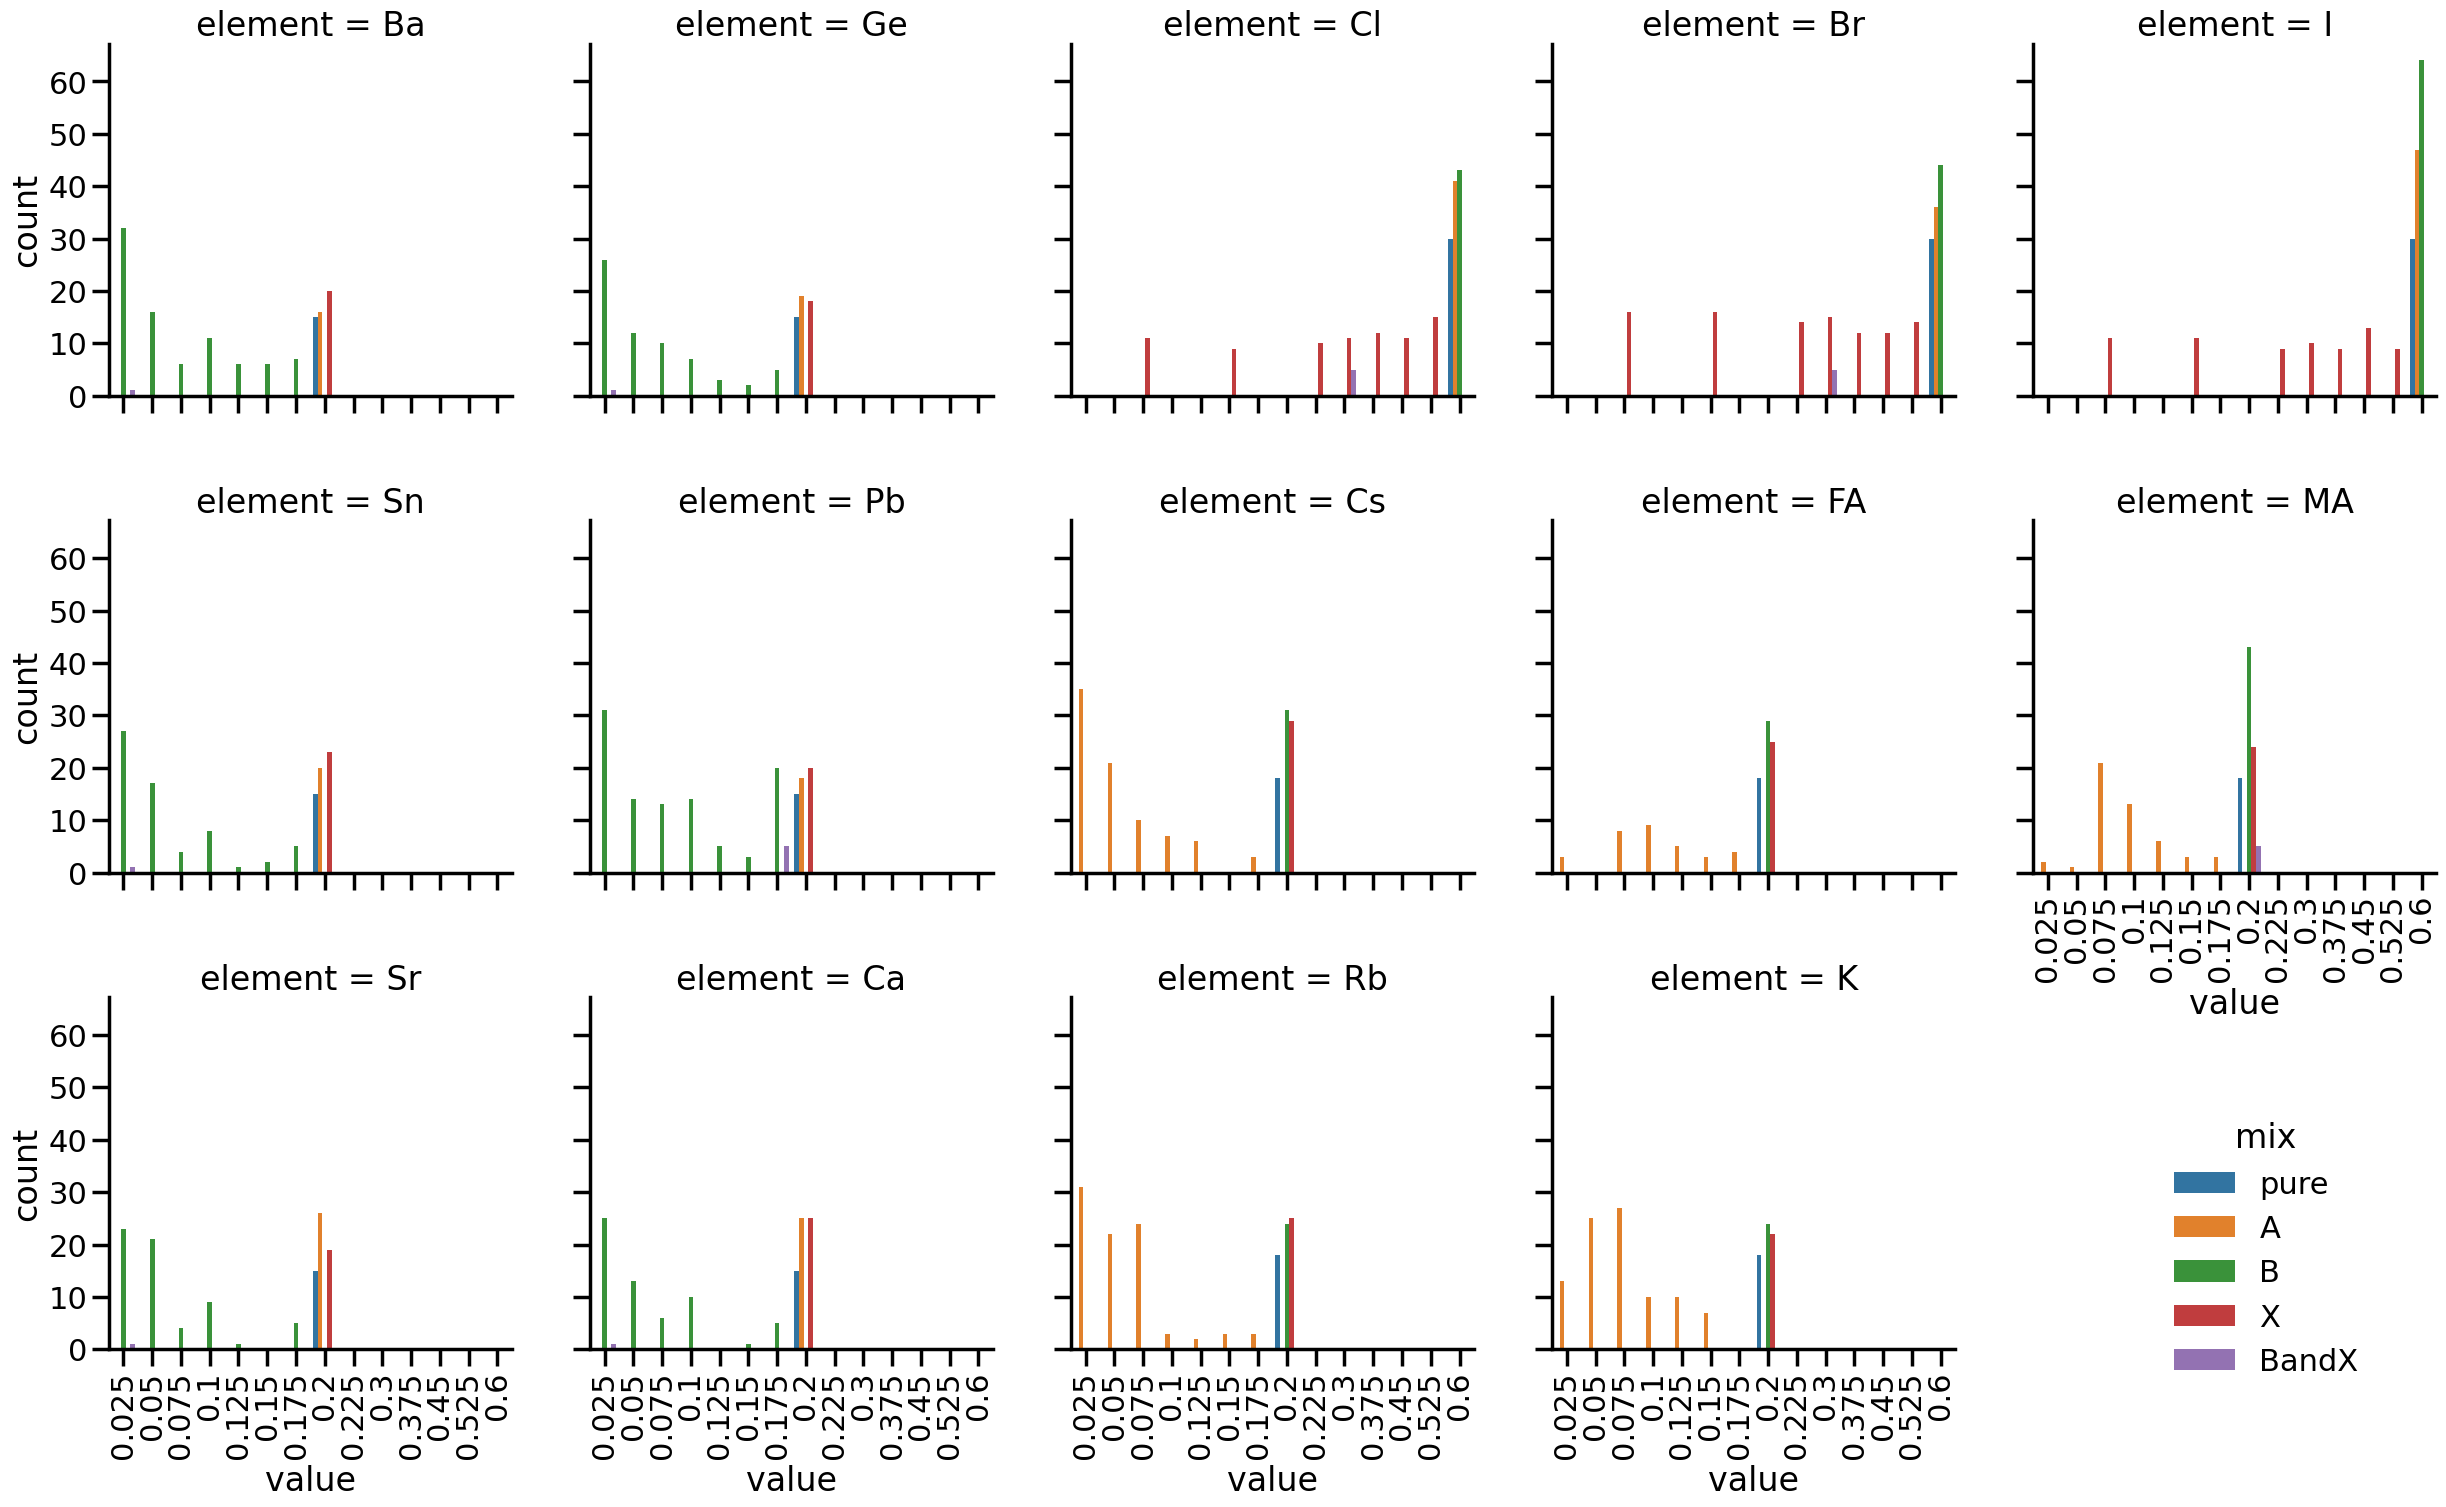
\includegraphics[width=.9\linewidth]{variability_of_composition_vectors.png}
\caption{\label{fig:chemspace_uni} Plots showing number of Perovskites representing a constituent at a certain atomic fraction of a complete Perovskite.}
\end{figure*}

\subsection*{{\bfseries\sffamily DONE} Calculation Details}
\label{sec:org7ac2ce4}
\begin{itemize}
\item State "DONE"       from "TODO"       \textit{[2022-06-06 Mon 17:17]}
\end{itemize}
DFT calculations are performed with \gls{vasp} version 6.2. The \acrlong{paw} potentials were used as pseudopotentials. The
\acrlong{gga} of \acrshort{pbe} and the hybrid \acrshort{hse}06
(\(\alpha\)=0.25 and \(\omega\)=0.2) functionals are used as
exchange-correlation energy. The energy cutoff for the plane-wave
basis is set to 500 eV. For \acrshort{pbe} the Brillouin zone was sampled by
6x6x6 reciprocal mesh using the Monkhorst-Pack k-point mesh. For \acrshort{hse}
the Brillouin zone was sampled by 2x2x2 reciprocal mesh using the
Monkhorst-Pack k-point mesh. The structural force convergence
threshold is set to be 0.005 eV/\AA{}.

\subsection*{{\bfseries\sffamily TODO} Discussion of DFT Computed Properties}
\label{sec:org3736488}
\begin{itemize}
\item State "DONE"       from "TODO"       \textit{[2022-06-06 Mon 17:19]}
\end{itemize}
\subsubsection*{{\bfseries\sffamily DONE} Decomposition Energy}
\label{sec:org792810a}
\begin{itemize}
\item State "DONE"       from "TODO"       \textit{[2022-06-06 Mon 00:43]}
\end{itemize}
The decomposition energy indicates the stability of a compound. To
calculate the decomposition energy for an ABX3 Perovskite, we assume
it will decompose to two phases, AX and BX2. Using \acrshort{dft} calculations,
we can get the optimized energy of a Perovskite and that of its
constituent phases. The decomposition energy is calculated using
equation \eqref{eq:decoE}. This calculation is performed separately for
each level of theory.

\begin{equation}\label{eq:decoE}
E_{decomp} = E_{opt}(ABX_3) - E_{opt}(AX) - E_{opt}(BX2)
\end{equation}

\subsubsection*{{\bfseries\sffamily TODO} SLME calculations}
\label{sec:org16d388b}
\begin{itemize}
\item State "DONE"       from "TODO"       \textit{[2022-06-06 Mon 17:30]}
\end{itemize}
The \gls{slme} metric developed by \citet{yu-2012-ident-poten} is used as the
primary criterion screening perovskites for their photovoltaic
merits. The \gls{slme} value is computed considering a 5\(\mu\)m absorption
layer for every Perovskite according to equation \eqref{eq:slme}.

\begin{equation}\label{eq:slme}

\end{equation}

This calculation is performed using Logan William's SL3ME
\cite{williams-2022-sl3me}. Based on absorption spectra obtained from
from \gls{vasp}. This calculation is performed separately for the \acrshort{pbe} band
gaps and the \acrshort{hse} band gaps, resulting in two synthetic efficiencies
for each record.

\section*{{\bfseries\sffamily TODO} Results and discussion}
\label{sec:org1ddd246}
\subsection*{{\bfseries\sffamily TODO} Visualization of DFT Data}
\label{sec:org5b69b03}
\begin{figure*}
\centering
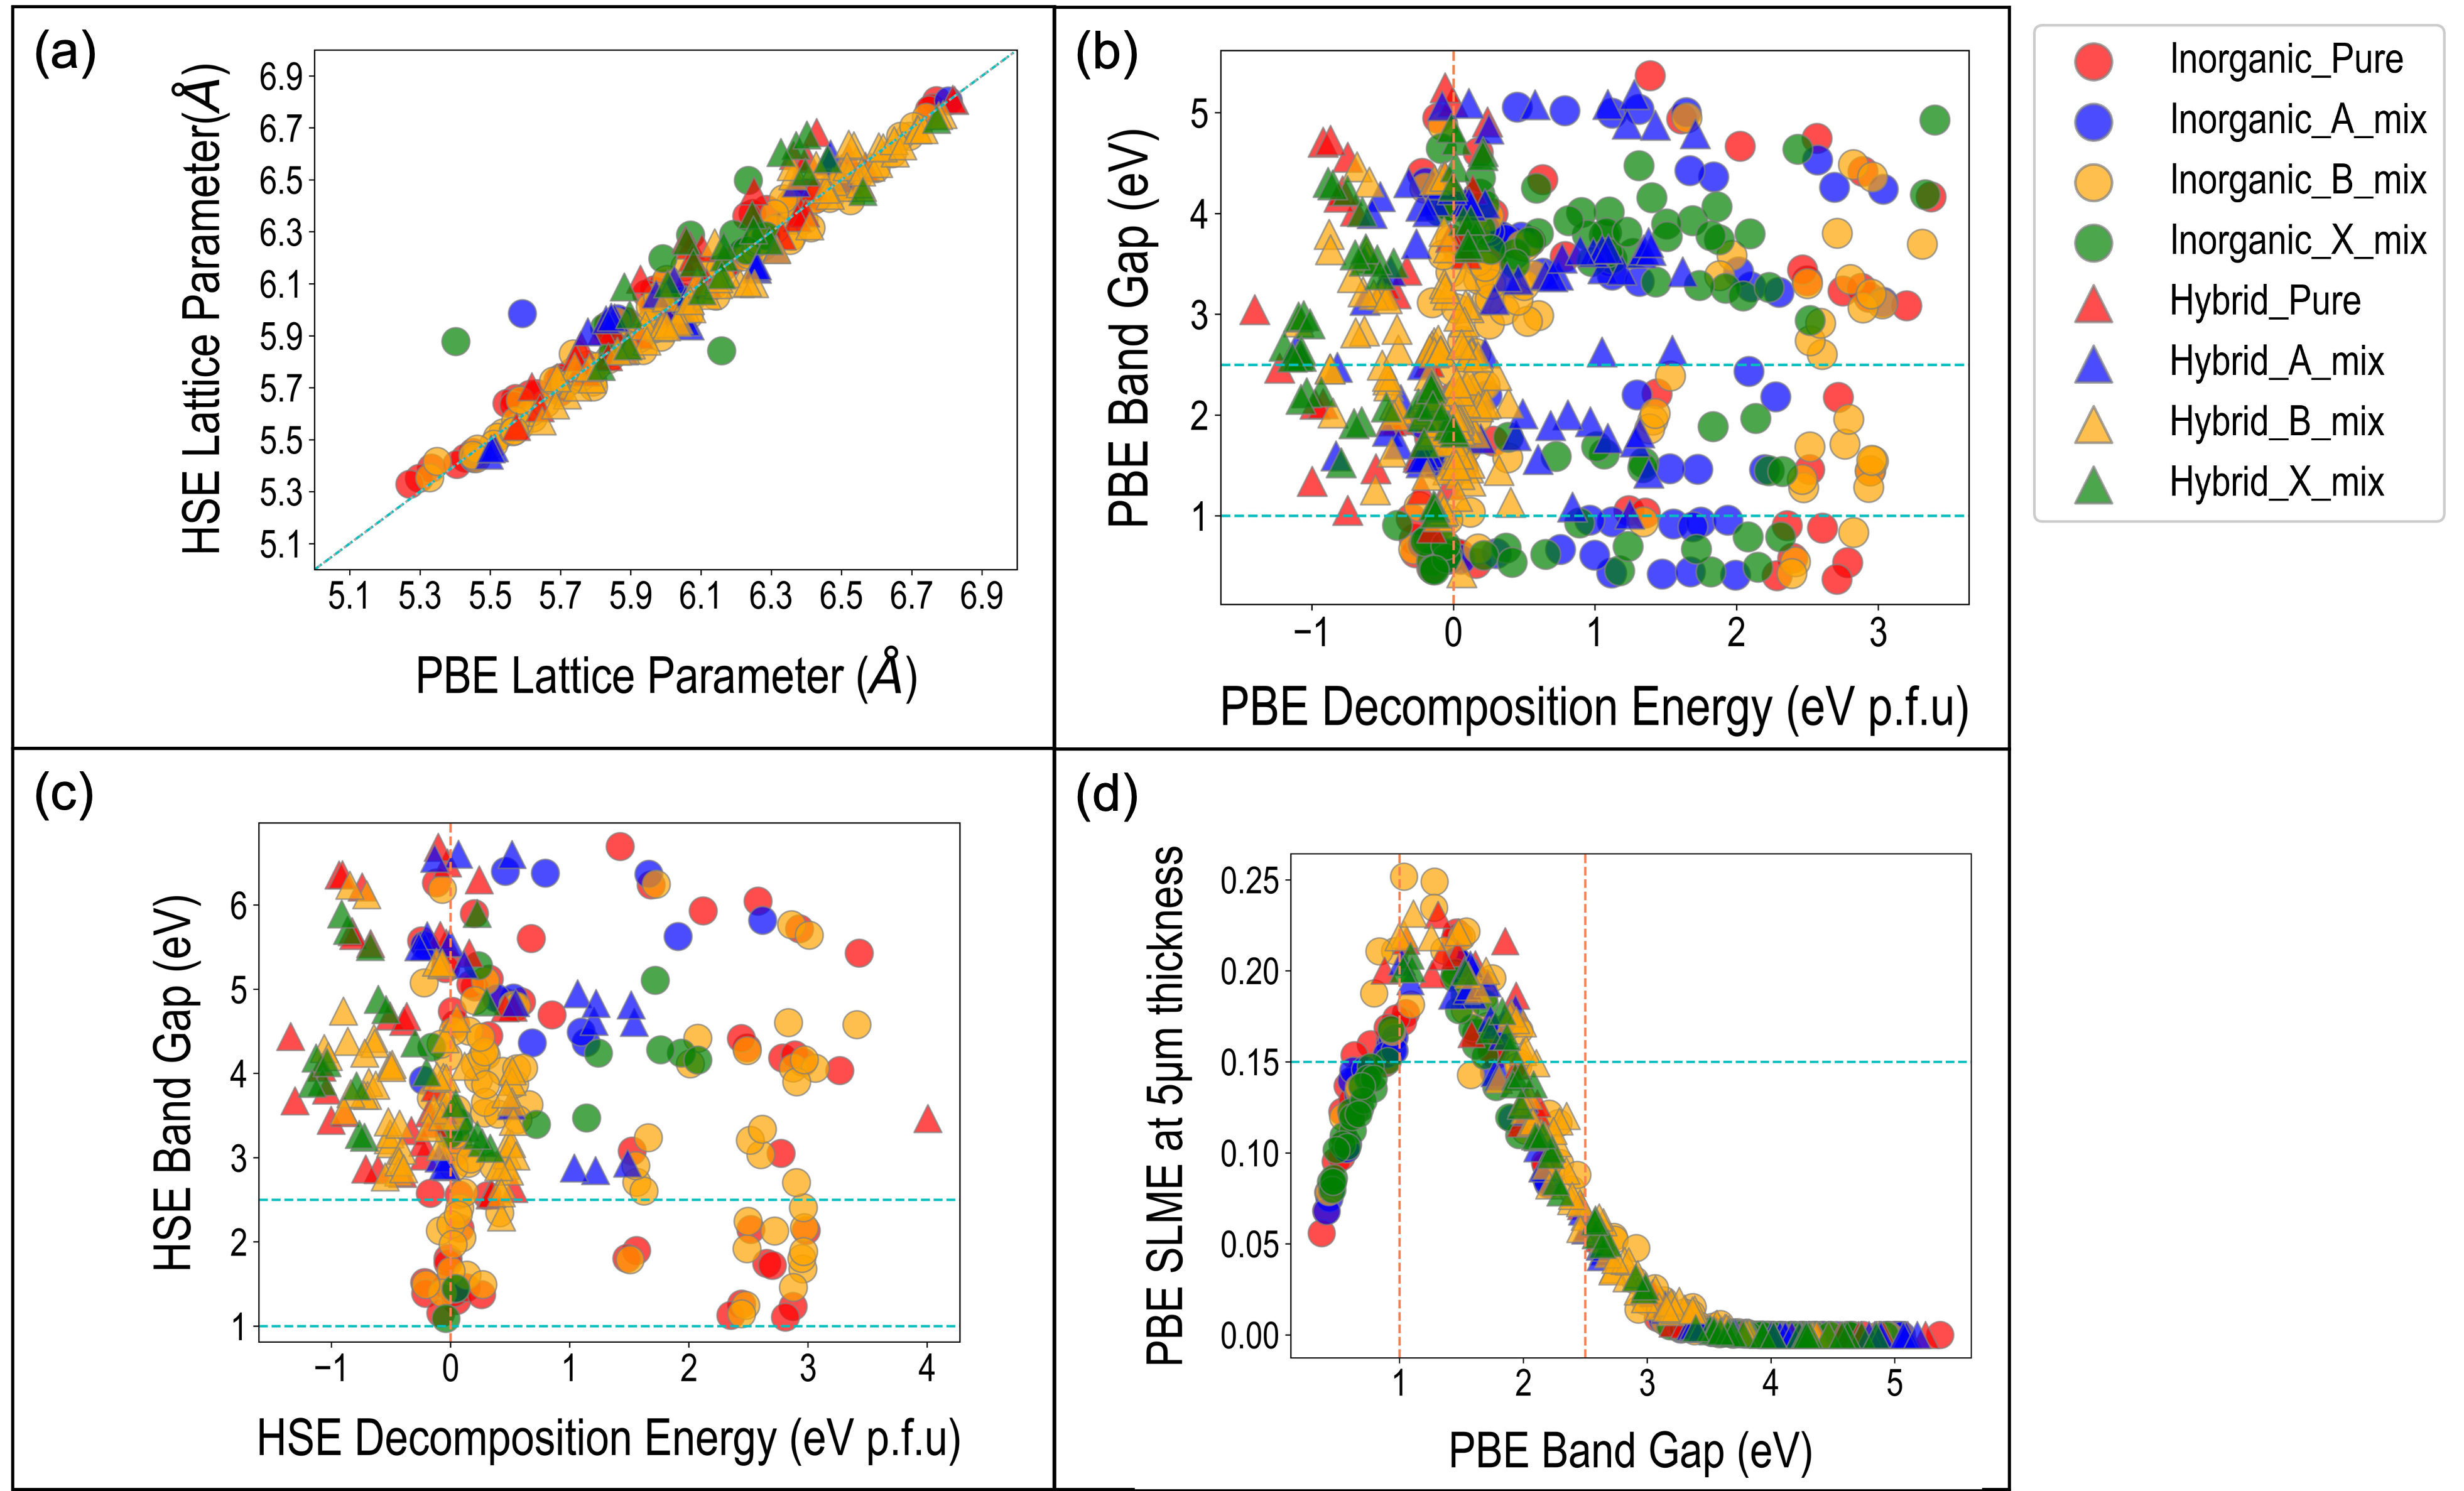
\includegraphics[width=.9\linewidth]{Figure2.png}
\caption{\label{fig:pairplots} DFT Results: PBE and HSE properties; lattice constants, decomposition energies, band gaps, and converter efficiencies.}
\end{figure*}

\subsubsection*{{\bfseries\sffamily DONE} Lattice constant PBE vs HSE}
\label{sec:org01f52c4}
\begin{itemize}
\item State "DONE"       from              \textit{[2022-06-06 Mon 01:02]}
\end{itemize}
Fig \ref{fig:lc_lot_vs} presents the lattice parameter comparison of
\acrshort{pbe} calculation and \acrshort{hse}
calculations. Full relaxations at both levels of theory mostly agree
on the lattice parameters. At least, any deviation appears to be very
linearly explained. This suggests the accuracy of
\acrshort{pbe} relaxation is enough to optimize most Perovskite
samples.

Note this also served as a reasonable validation for our results. A
few samples did have significantly differing lattice parameters. This
prompted checking the optimized structures. We found those Perovskite
structures were substantially deformed and no longer had obvious
octahedral structures. Thus, we exclude these outliers from any
analysis concerned with the dominant pseudo cubic structures which are
the focus of this report.

\begin{center}
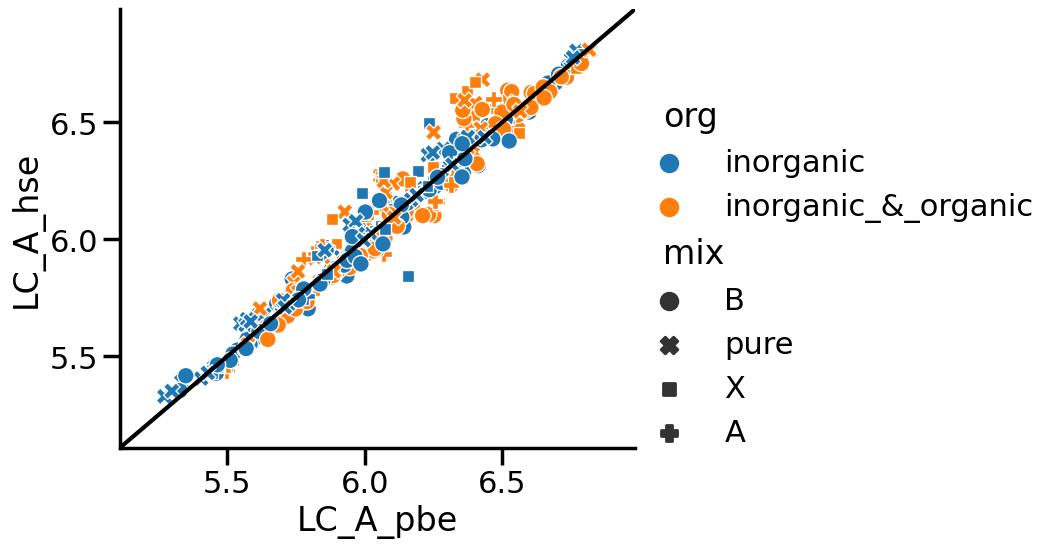
\includegraphics[width=.9\linewidth]{pbe_v_hse_LC.png}
\captionof{figure}{\label{fig:lc_lot_vs} Comparing lattice constants obtain by full PBE and HSE relax calculations}
\end{center}

\subsubsection*{{\bfseries\sffamily TODO} Comparing synthetic to physical data}
\label{sec:org384c7c0}
\begin{itemize}
\item State "DONE"       from              \textit{[2022-06-06 Mon 01:01]}
\end{itemize}
\begin{center}
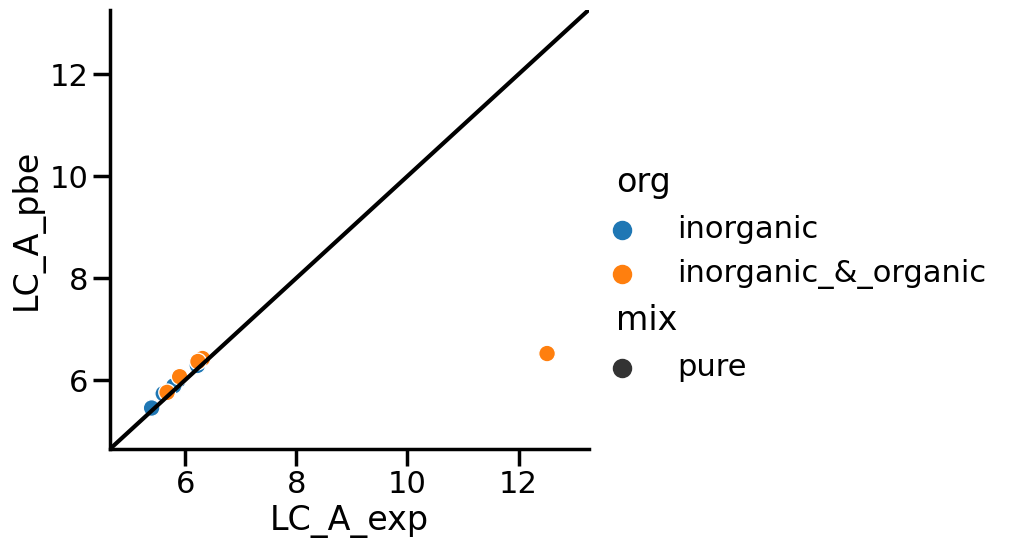
\includegraphics[width=.9\linewidth]{pbe_v_exp_LC.png}
\captionof{figure}{\label{fig:lc_val_vs} Comparison of PBE and HSE computed pseudo-cubic lattice constants with crystallographic measures for lattice constants}
\end{center}
\begin{center}
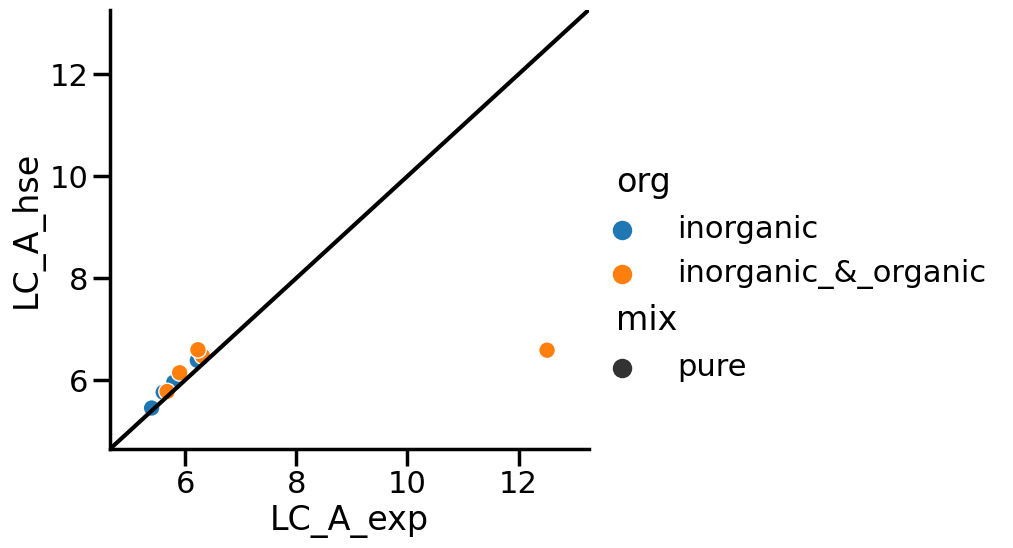
\includegraphics[width=.9\linewidth]{hse_v_exp_LC.png}
\captionof{figure}{\label{fig:lc_val_vs} Comparison of PBE and HSE computed pseudo-cubic lattice constants with crystallographic measures for lattice constants}
\end{center}

The physical data used in comparison is collected from the works of
\citet{briones-2021-accel-lattic,jiang-2006-predic-lattic,chen-2015-under-spotl}.

The synthetic lattice constants do mostly agree with experiment. The
\acrshort{pbe} lattice constants are better than the \acrshort{hse} measures \ref{tbl:verror}.

It should be noted that the physical \acrshort{fa}SnI\textsubscript{3} measure reported by
\citet{chen-2015-under-spotl} is clearly an orthorhombic phase. The
validating lattice constant here is obtained by averaging lattice
parameters. However, per the \hyperref[sec:org70ec3ea]{Deviation from Cubicity} metric, this
phase is still approximately cubic, with angles near enough to 90
degrees that we consider the data point valid. However, this does
explain the disagreement in the parity plots.

\begin{table}[htbp]
\caption{\label{tbl:verror} Root Mean Squared Error}
\centering
\begin{tabular}{ll}
HSE v EXP & PBE v EXP\\
\hline
 & \\
\end{tabular}
\end{table}

\subsubsection*{{\bfseries\sffamily TODO} Decomposition energy vs band gap PBE and HSE}
\label{sec:orgec1495c}
Fig 2(b) is showing the \acrshort{pbe} band gap compared to the
\acrshort{pbe} decomposition energy. It presents the diversity
of our Perovskite dataset. The data sets cover a large range of band
gap and decomposition energy. For example, we have Perovskite with low
decomposition energy (good stability) and suitable band gap value
(between 1 eV to 2.5 eV for \acrshort{pbe} calculations). And
we can also find samples with low stability and large band gap. The
distribution of band gap and decomposition energy shows a great
diversity of all Perovskite samples and indicates that our data set
can statistically represent a sufficient Perovskite space. Fig 2(c)
shows the plot of \acrshort{pbe} band gaps and
\acrshort{hse} decomposition energy. Since we applied
\acrshort{hse} calculations for part of the samples, it shows
some grouping on low decomposition energy. Compared to
\acrshort{pbe} plot, more data should be added in high
decomposition energy region and suitable band gap region.

\subsubsection*{{\bfseries\sffamily TODO} Spectroscopic Limited Maximum Efficiency (SLME) vs PBE Band gap}
\label{sec:org4842677}
Fig 2(d) presents the \gls{slme} values related to the
\acrshort{pbe} band gap. \gls{slme} is a proven proxy
for photovoltaic performance
\cite{yu-2012-ident-poten}. \gls{slme} measures the
absorption efficiency of light for the Perovskite. As Fig 2(d)
showing, a peak around 1.5 eV is obvious. The peak indicates that
these samples with 1.5 eV \acrshort{pbe} band gap will also
have best absorption efficiency as photovoltaic materials. As the band
gap increases, the \gls{slme} value decreases and eventually
goes to zero due to the high band gap values.

\subsection*{{\bfseries\sffamily TODO} Pearson Correlation Results}
\label{sec:org3babf08}
\begin{figure*}
\centering
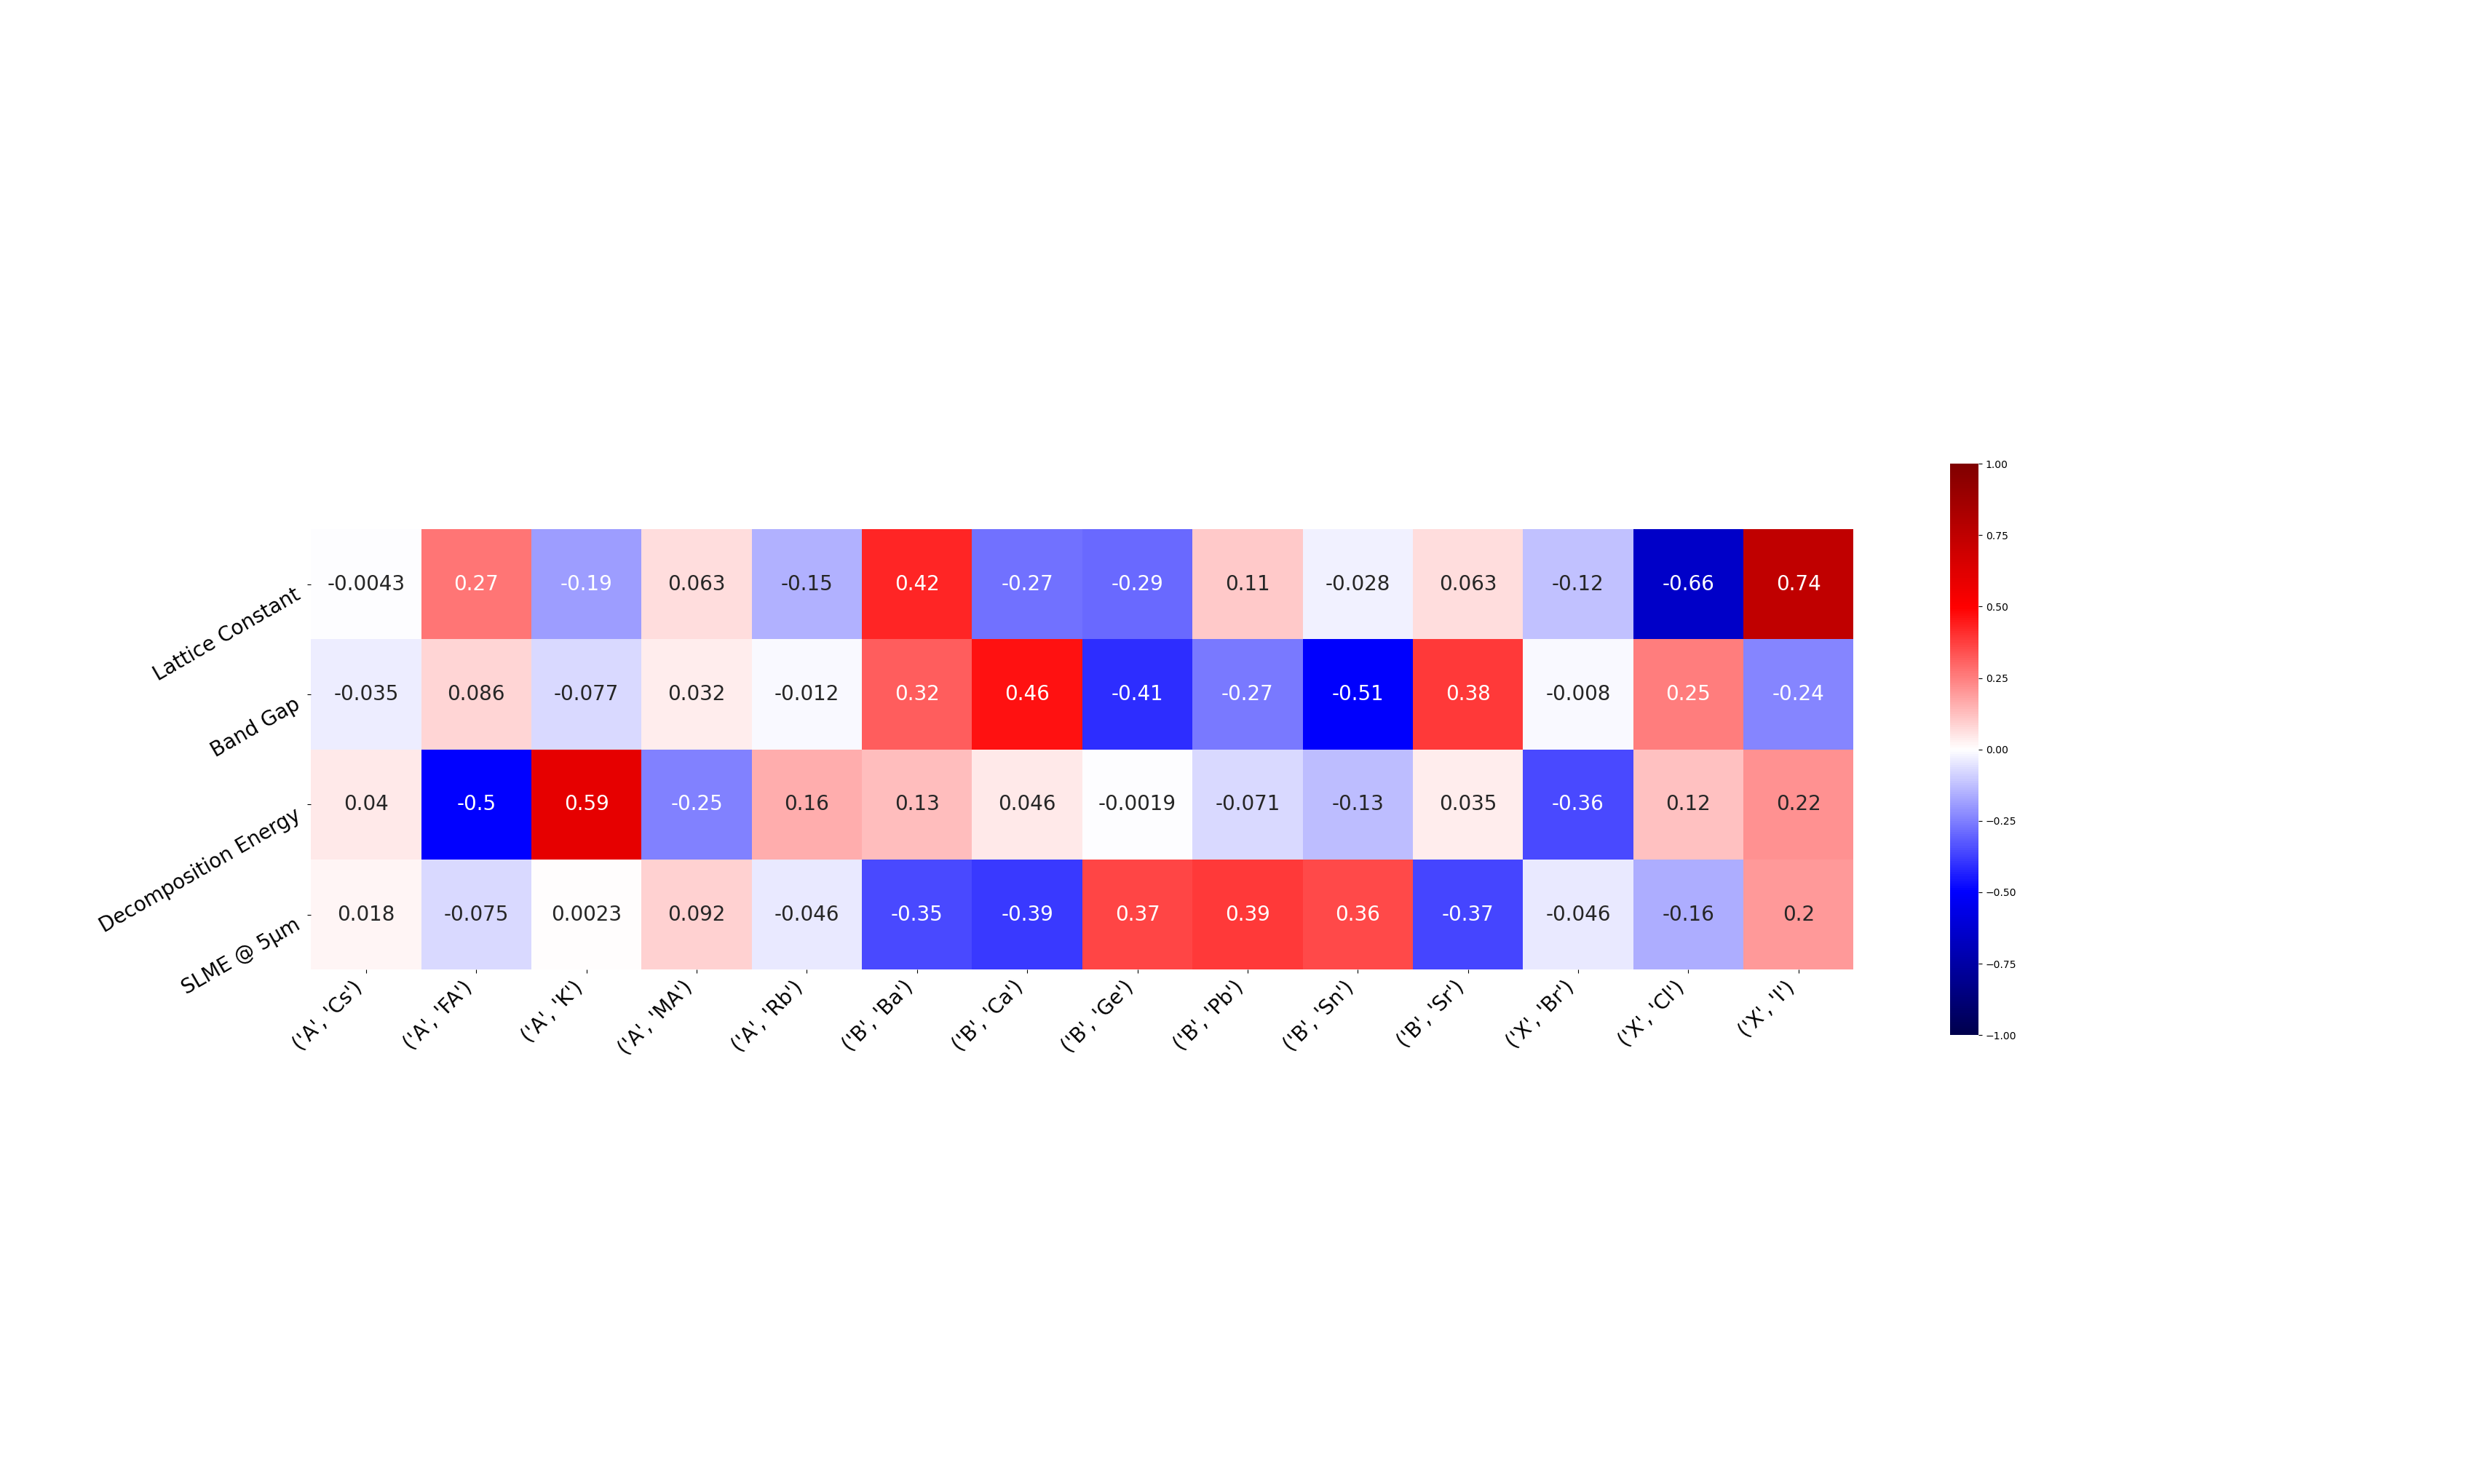
\includegraphics[width=.9\linewidth]{PBE_v_comp_pearson2.png}
\caption{\label{fig:pearson_pcomp} Pearson linear correlation coefficients between 14 composition variables, and 4 PBE computed properties}
\end{figure*}

\begin{figure*}
\centering
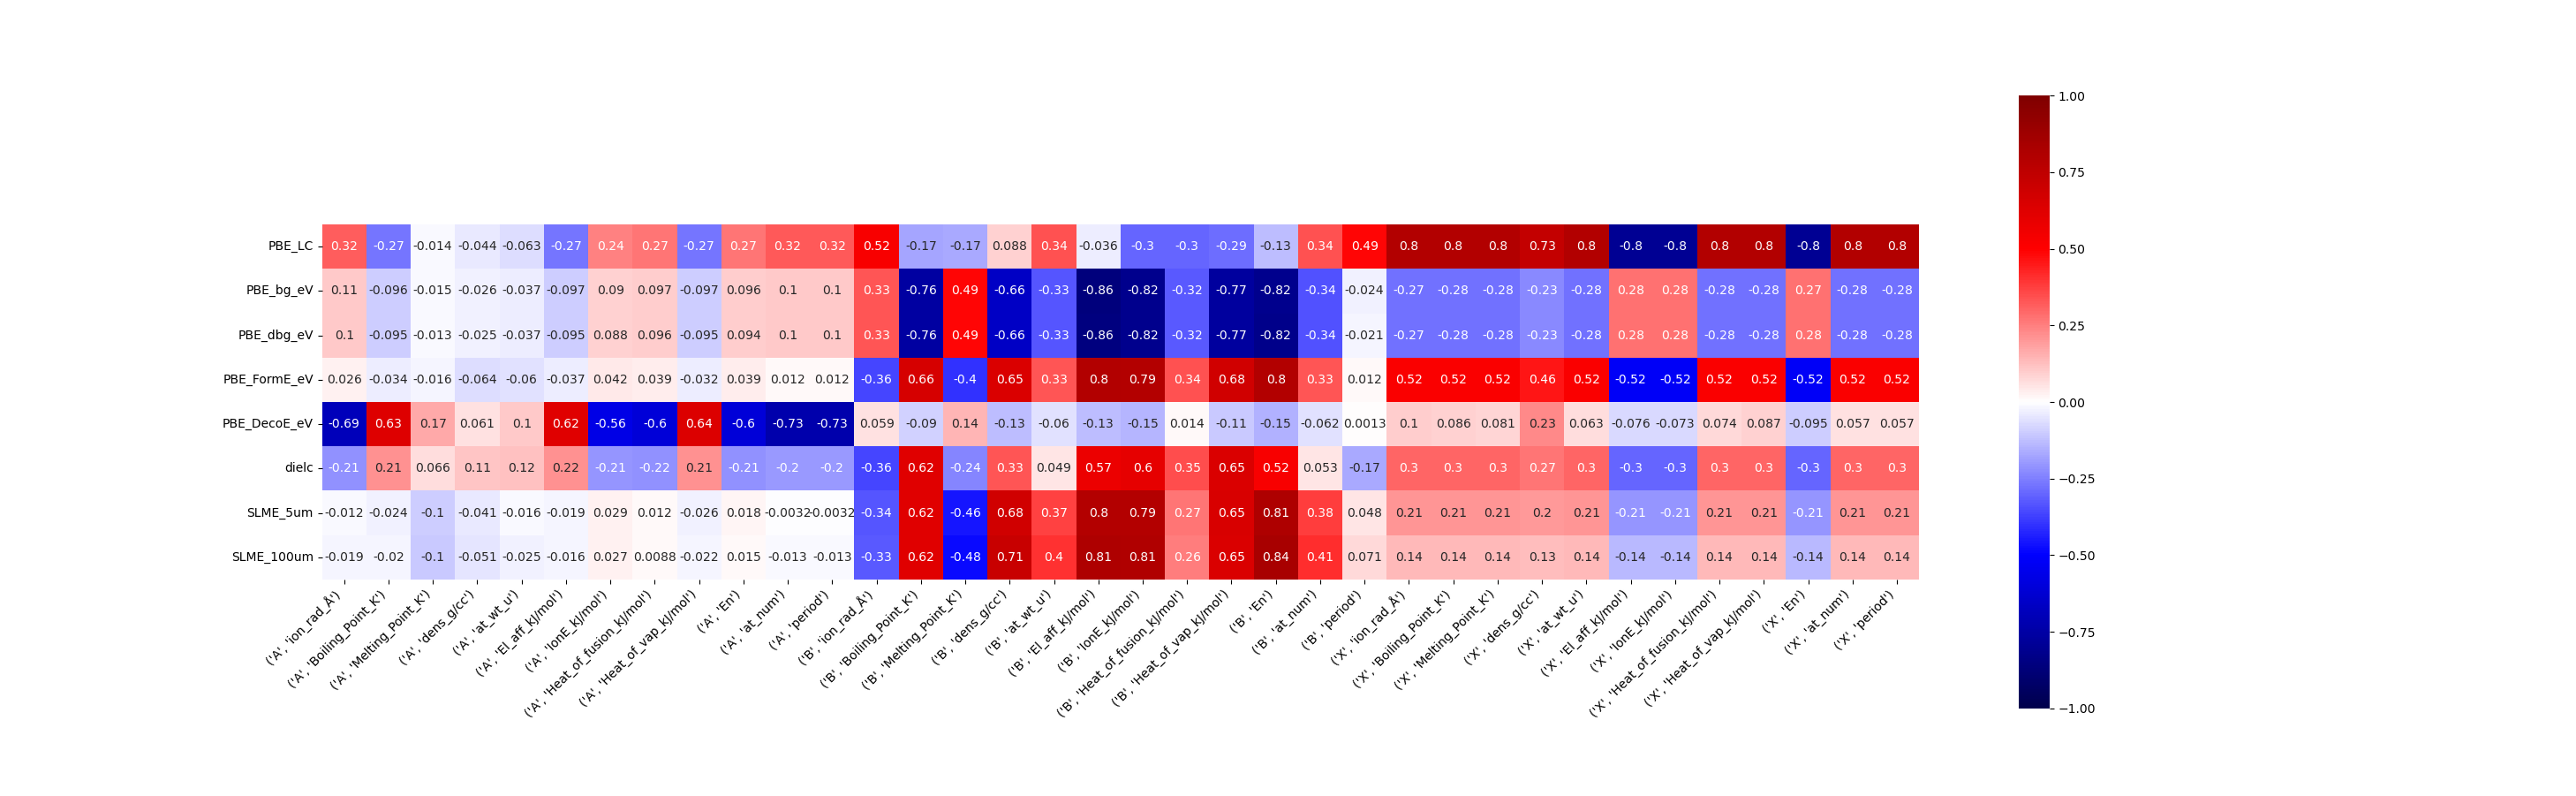
\includegraphics[width=.9\linewidth]{PBE_v_site_prop_pearson.png}
\caption{\label{fig:pearson_psite} Pearson linear correlation coefficients between 36 elemental descriptors and 4 PBE computed properties}
\end{figure*}

No target is adequately explained by a single composition or
composition derived axis. But there are helpful relations that aid
understanding the significance of key composition derived descriptors.

A Pearson correlation map is produced to check for strong
relations. Those that exist, when plotted in detail show some
trending, but always with extensive variability. Evidently, an
accurate model will have to be formed on a multidimensional domain.

\subsection*{{\bfseries\sffamily TODO} PCA}
\label{sec:org060b7fd}
\begin{figure*}
\centering
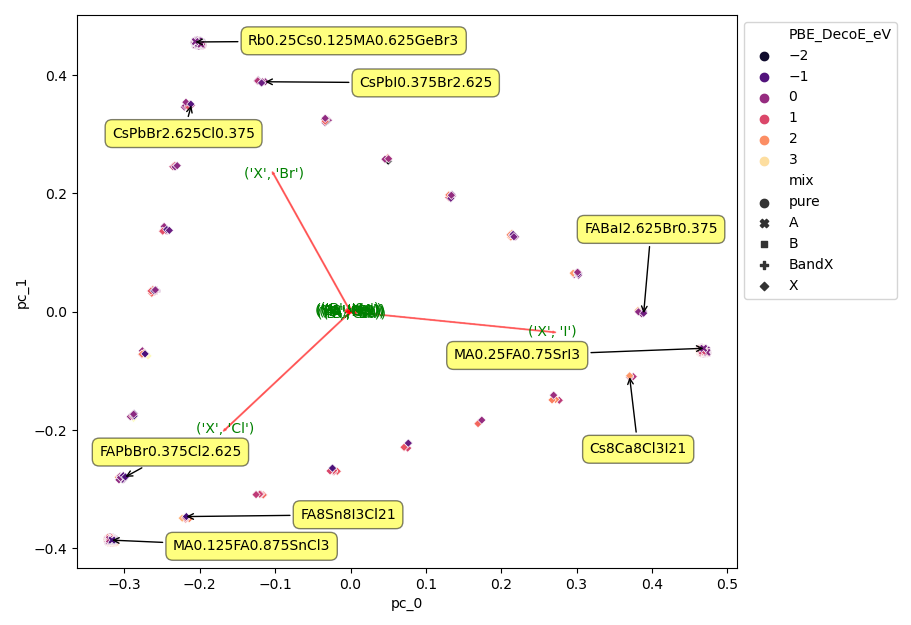
\includegraphics[width=.9\linewidth]{comp_ratio_projection_annot.png}
\caption{\label{fig:pca} PCA}
\end{figure*}

\gls{pca} is a method of projecting high dimensional data onto
a plane defined by the two linear combinations of axes that explain as
much of the variance as possible.

The method of \gls{pca} is the Singular Value Decomposition, a
Unitary Transform which generalizes the familiar
eigendecomposition. \gls{pca} will "rotate" the N data points
in M-D space until their widest 2D cross section is displayed.

At this point it is readily apparent that this dataset is highly
topological. The data exists on a mostly bounded domain in high
dimensions, so there is some geometry the features constitute.

Our models will prefer to use this this geometric structure in their
explanation for why Perovskite properties vary, this can be useful for
accuracy, it can also be a bias-inducing hindrance.

\subsection*{{\bfseries\sffamily TODO} t-SNE visualization of stability clustering}
\label{sec:org1c2e23d}
\begin{figure*}
\centering
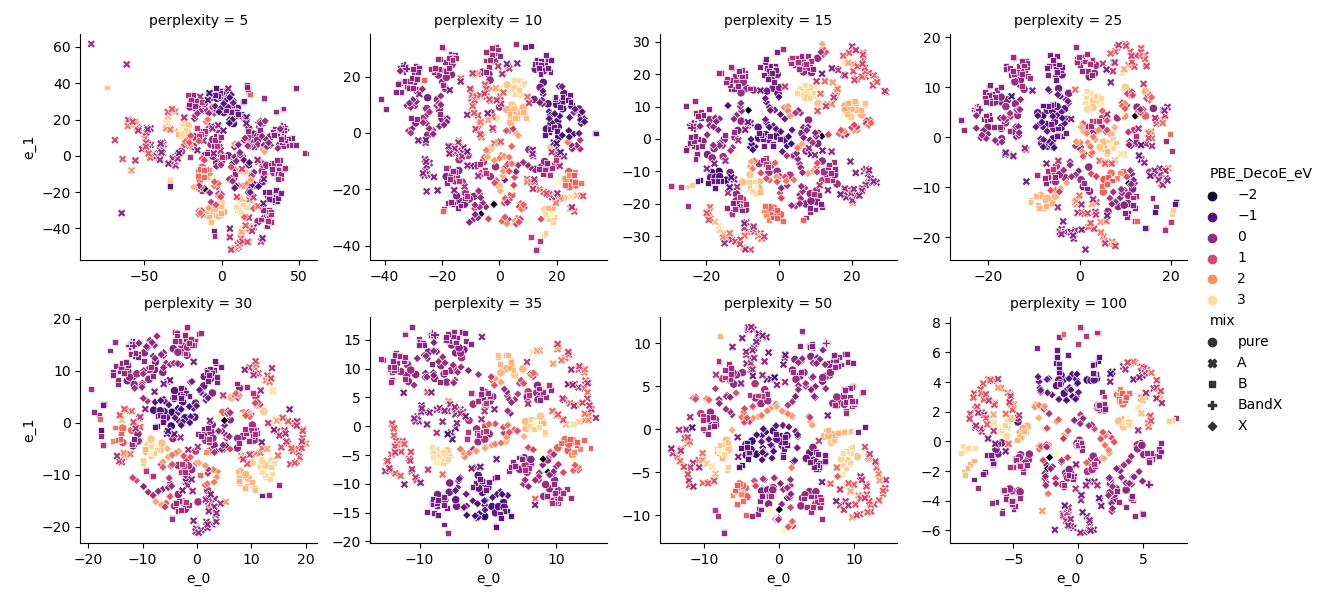
\includegraphics[width=.9\linewidth]{tsne_comp_DecoE_clusters.png}
\caption{\label{fig:tsne} t-SNE}
\end{figure*}

\subsection*{{\bfseries\sffamily DONE} Screening process of all samples in database}
\label{sec:orga576afc}
\begin{itemize}
\item State "DONE"       from              \textit{[2022-05-24 Tue 13:31]}
\end{itemize}
The synthetic Perovskite data is collected for sampling variety and
without regard for each compound's viability. In order to extract
potentially high-performing candidates for synthesis, we screen all
samples according to certain constraints, thereby obtaining some
Perovskites worth examining with higher Level of Theory
\acrshort{dft} calculations and future physical experiments by
brute force. This dataset can only confidently claim to sample cubic
phase perovskites. Therefore, a promising candidate should have low
deformation. Additionally, a lower decomposition energy combined with
a maximal \gls{slme} value would be ideal for physical
testing. Our screening procedure consists of cutting based on a custom
Deviation from Cubicity metric, octahedral factor, Goldschmidt
tolerance factor, Bartel tolerance factor, decomposition energy, and
band gap -- acting as less stringent proxy for the \gls{slme}
spectrum. The following sections will discuss the details of each
constraint.

\begin{figure*}
\centering
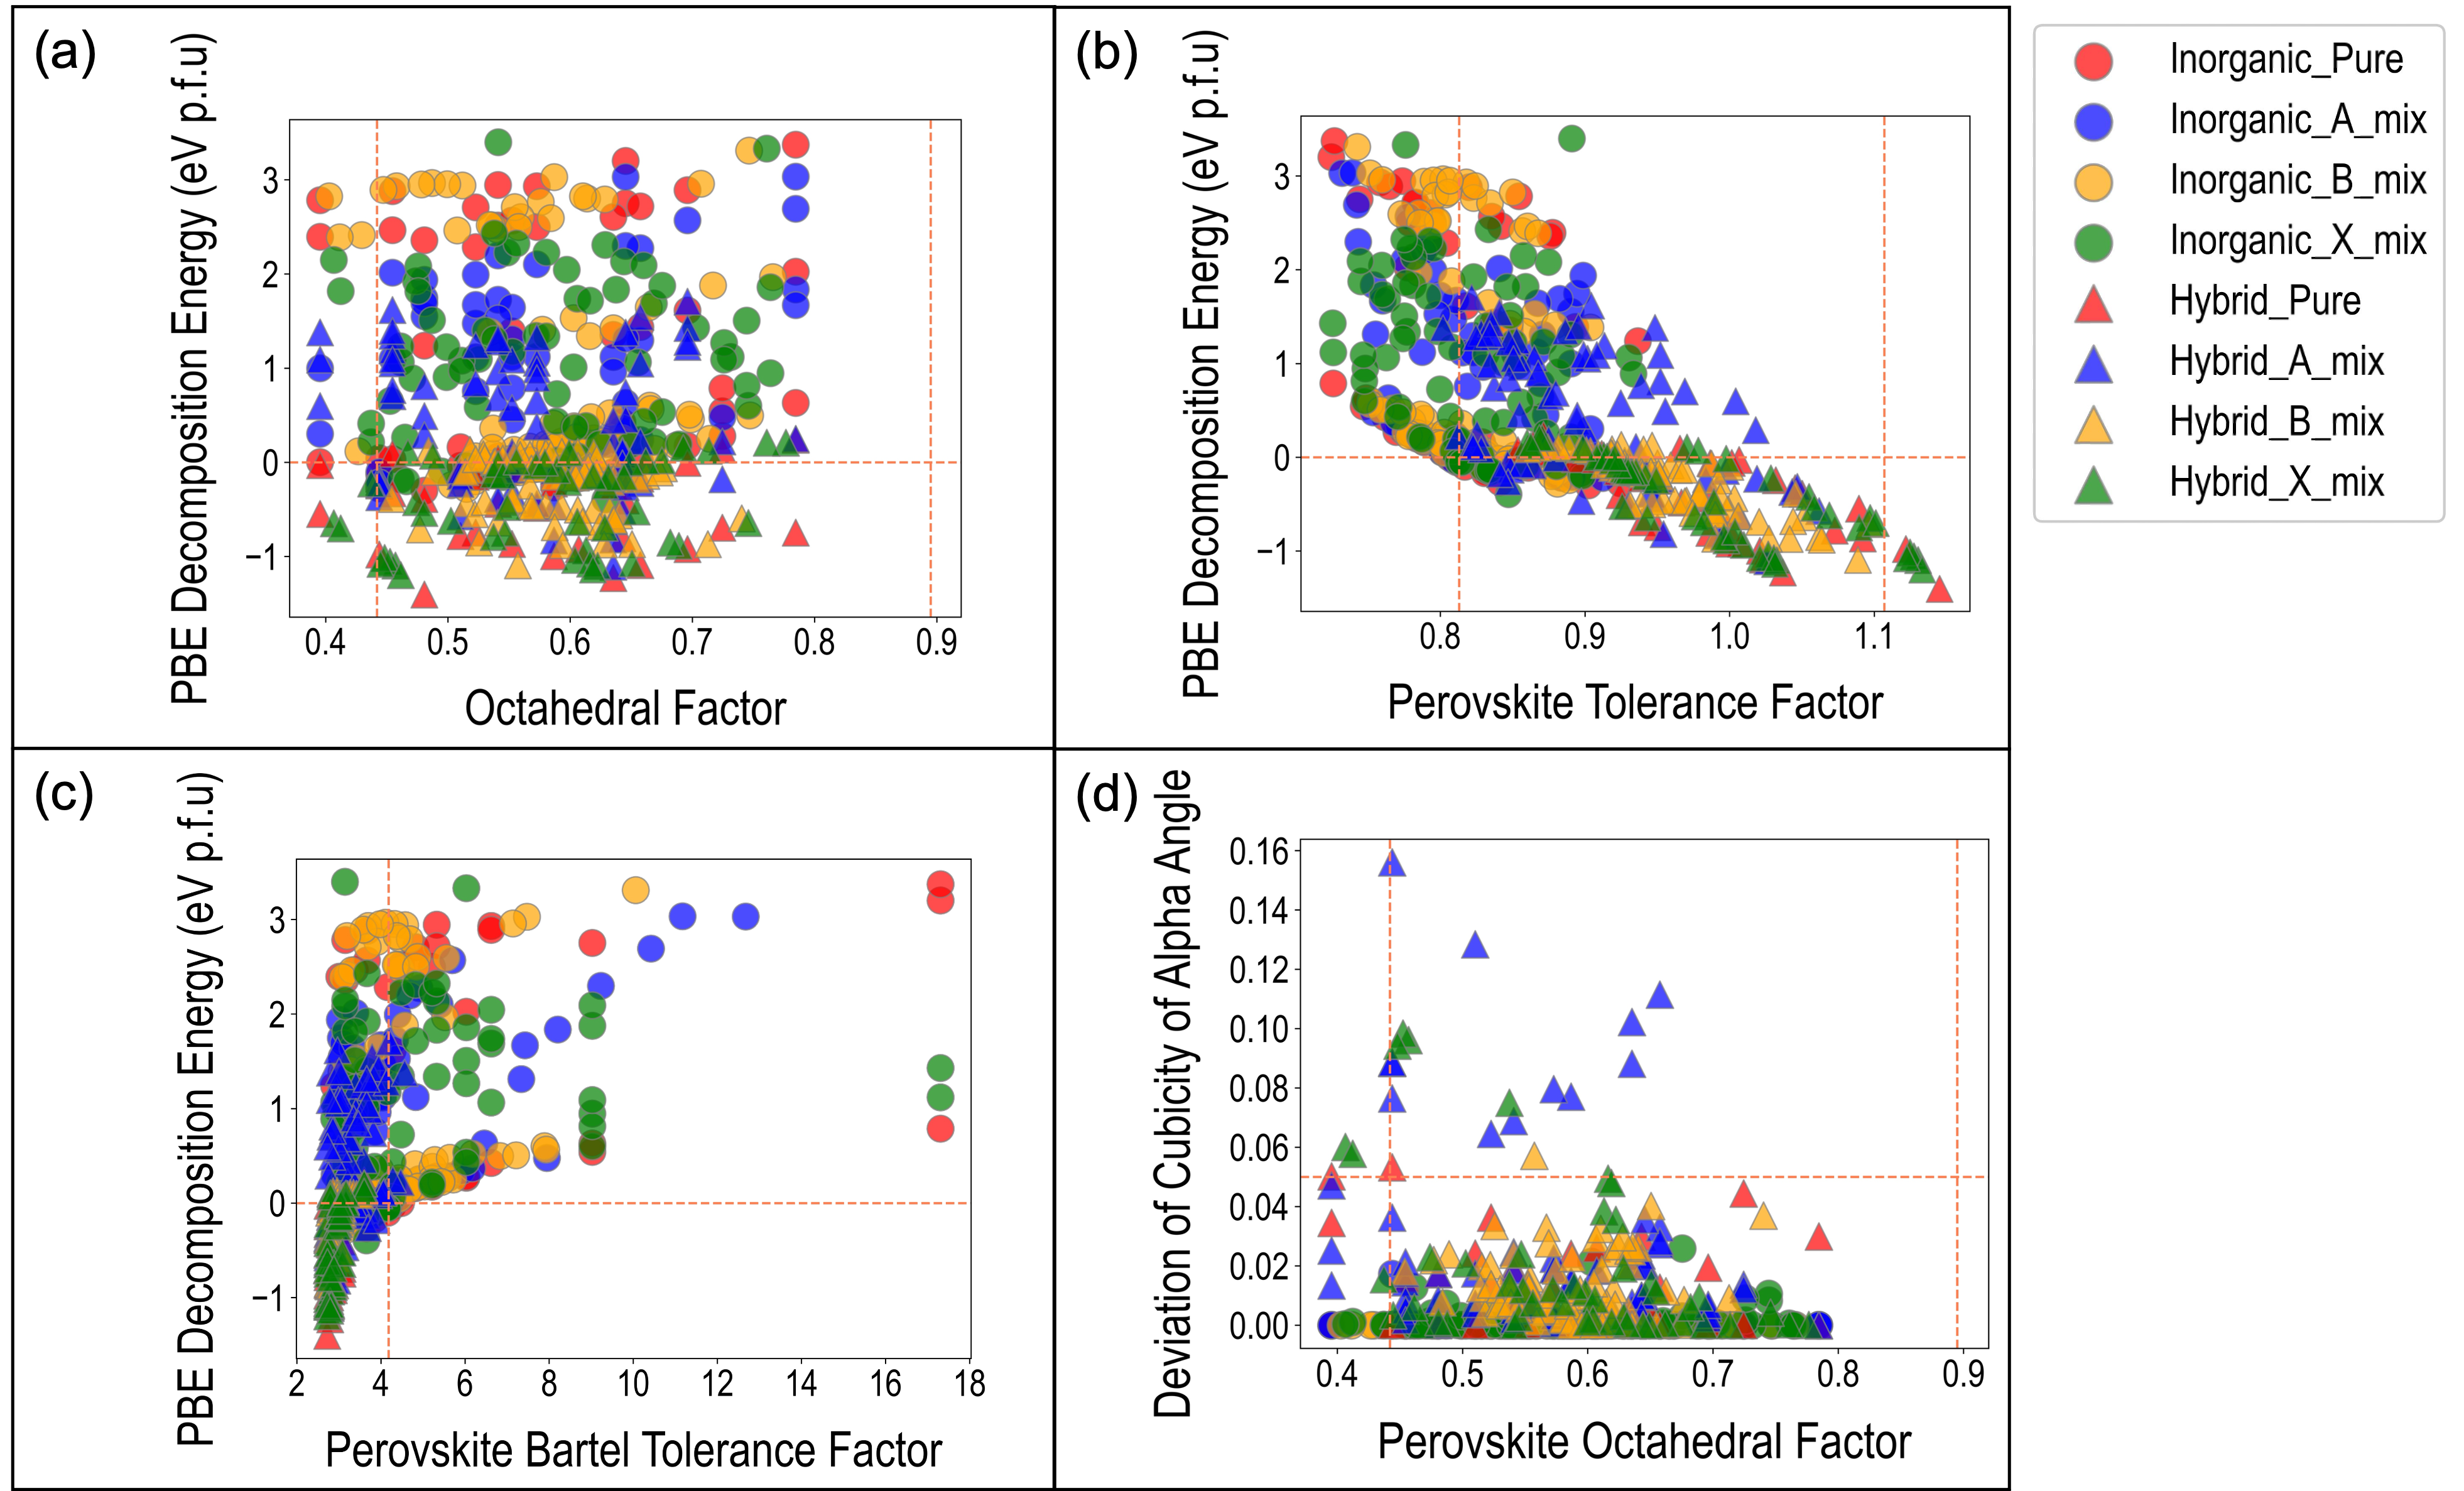
\includegraphics[width=.9\linewidth]{screening_factor.png}
\caption{\label{fig:cuts} Screening results of Decomposition Energy for (a) octahedral factor (b) Tolerance Factor (c) Bartel Tolerance Factor (d) Deviation of Cubicity.}
\end{figure*}

\begin{figure*}
\centering
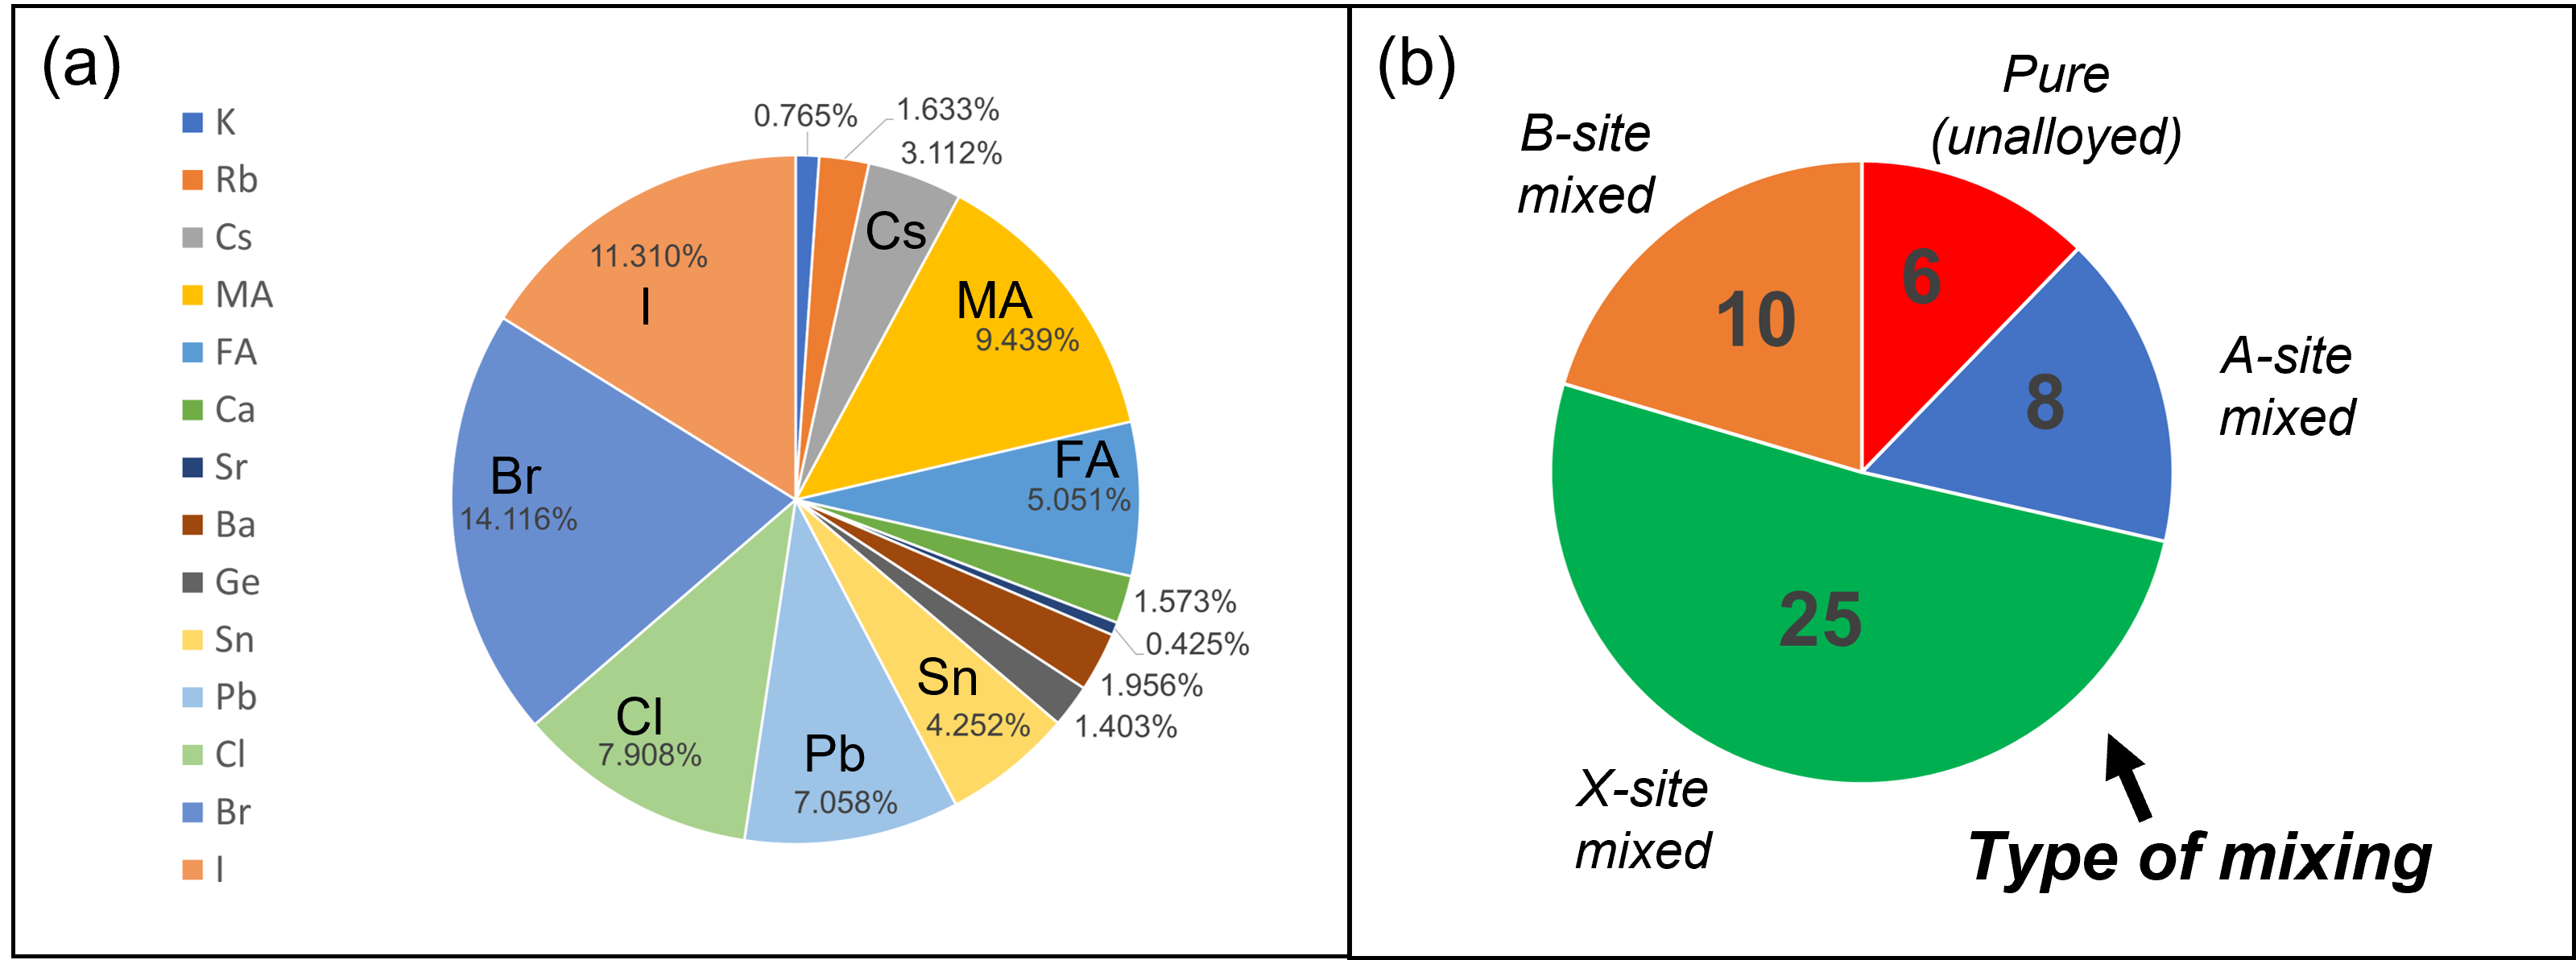
\includegraphics[width=.9\linewidth]{screening_pie.png}
\caption{\label{fig:leftover} 49 Screened perovskites analysis, (a) pie chart of element distribution, (b) pie chart of site mixing}
\end{figure*}

\begin{figure*}
\centering
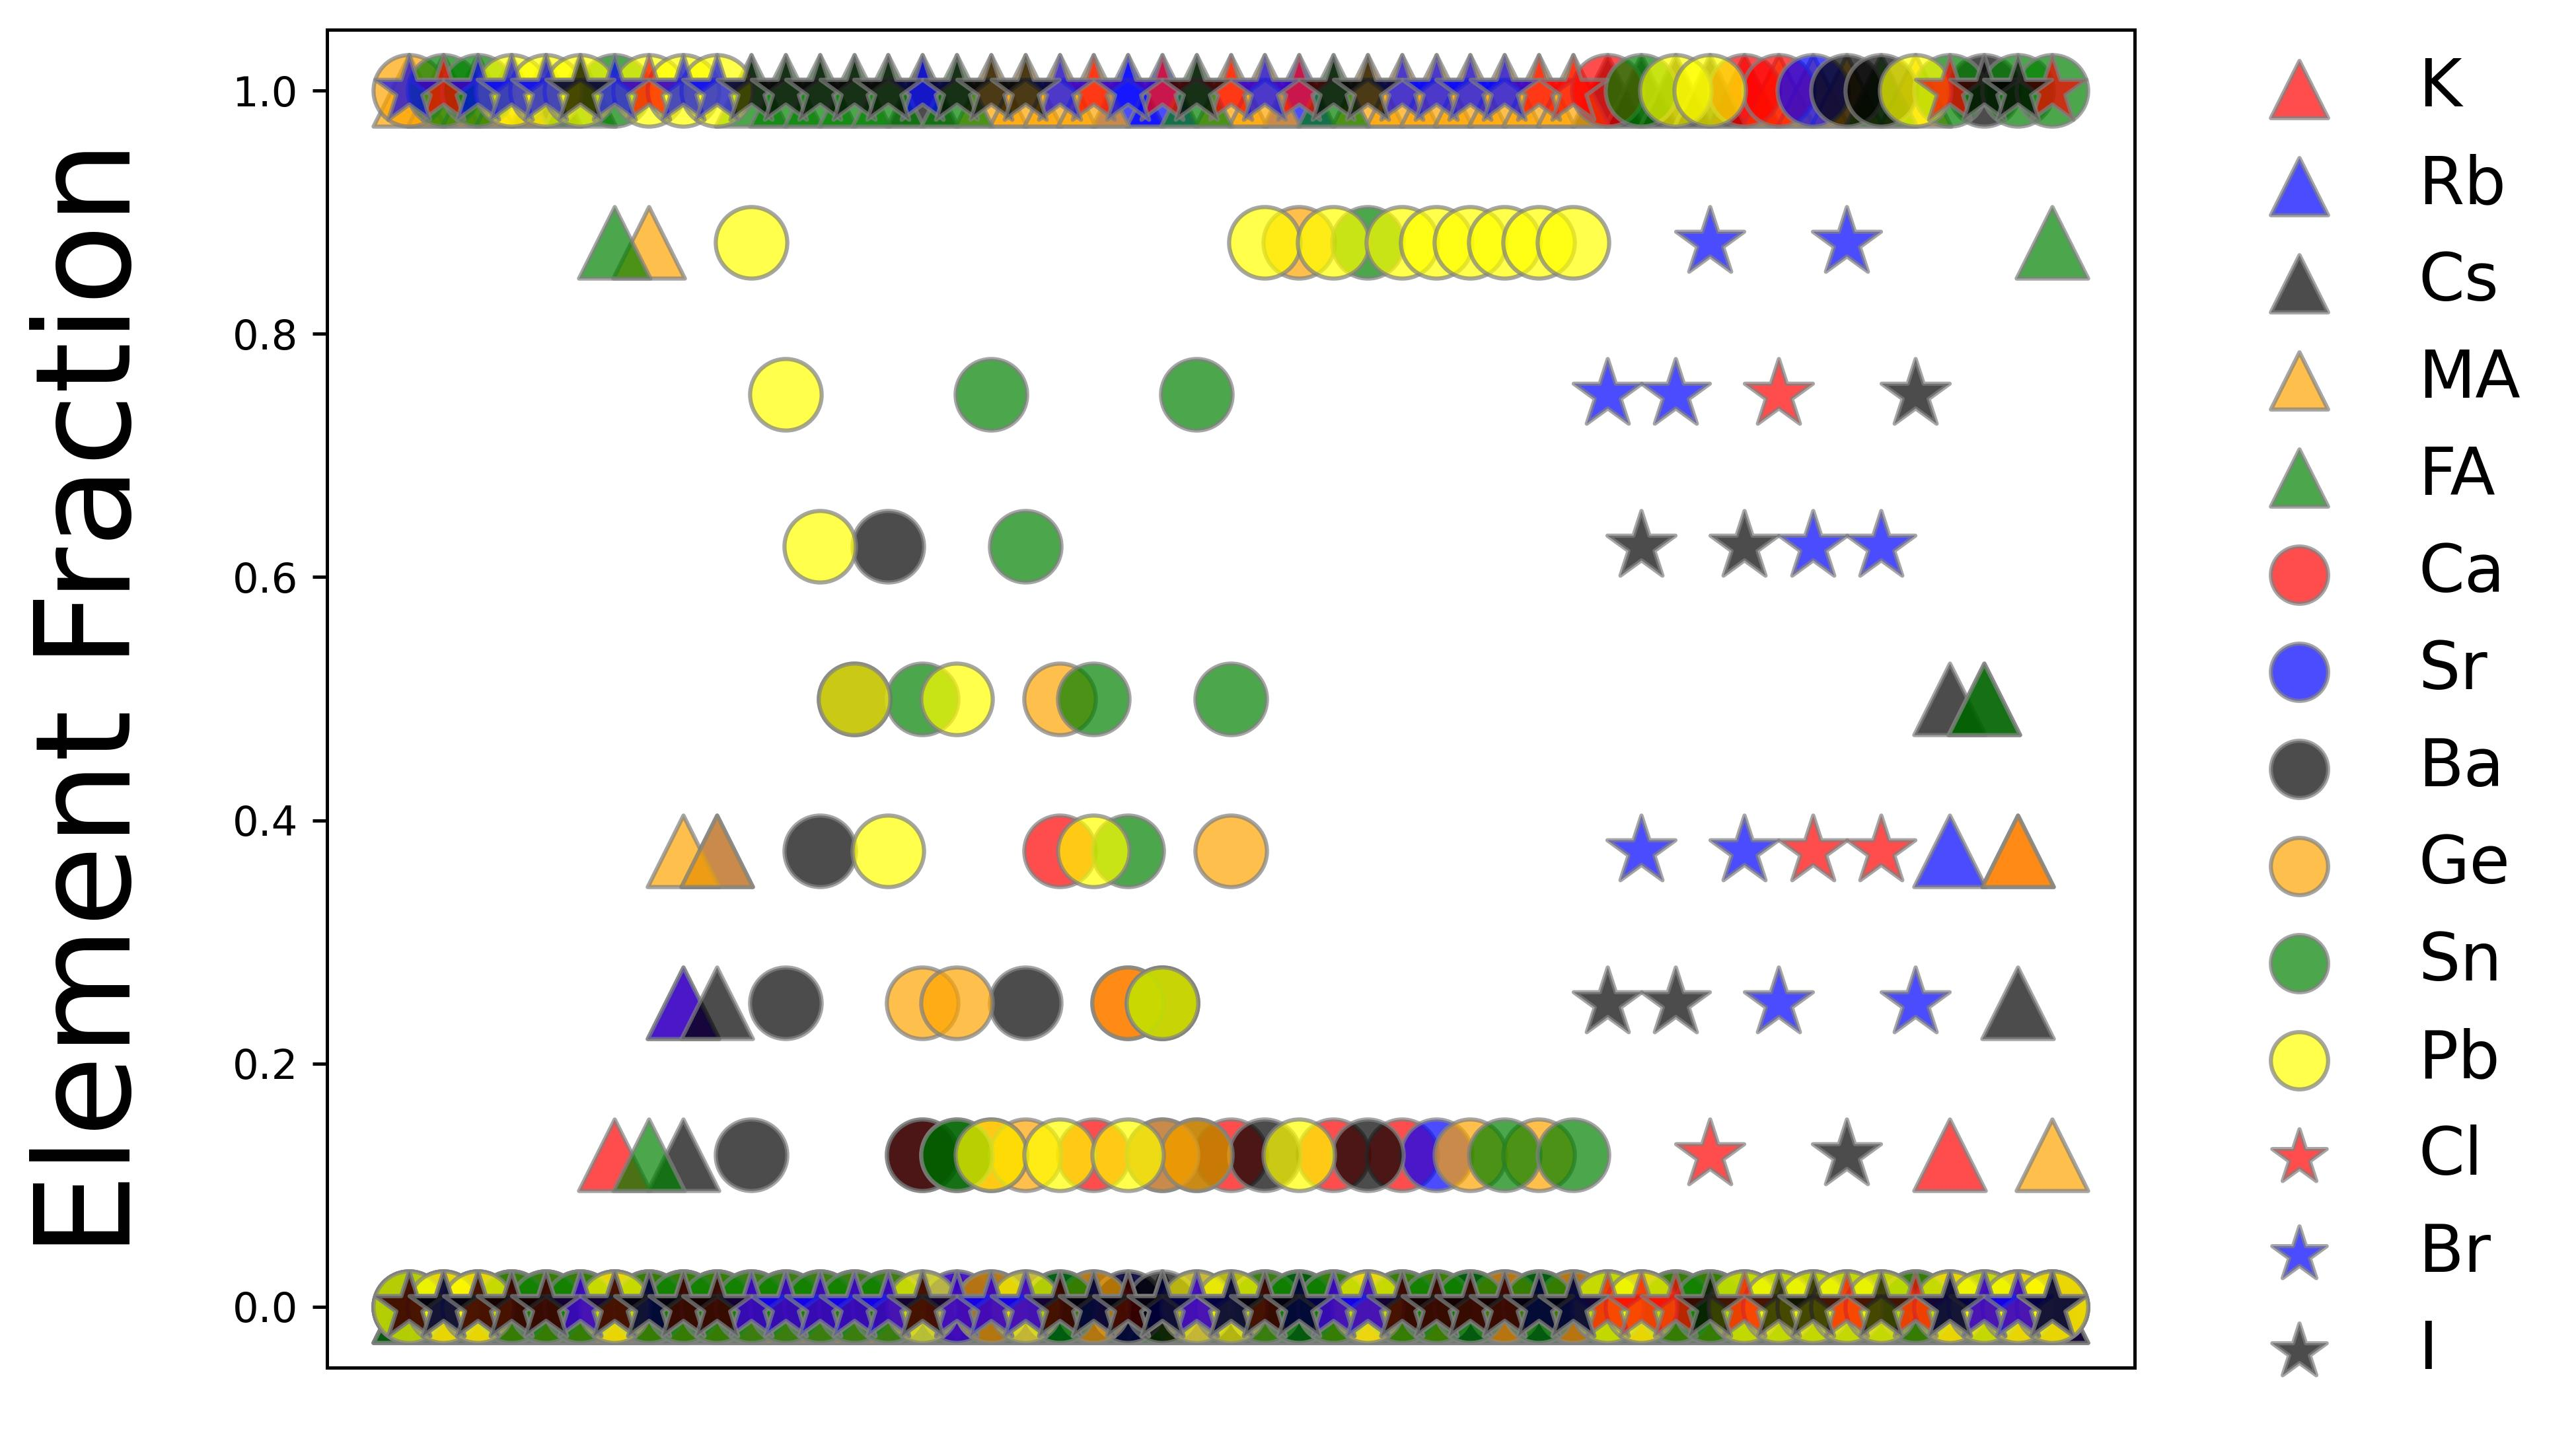
\includegraphics[width=.9\linewidth]{Element_Frac.jpg}
\caption{\label{fig:leftover_comp} Plots of element fraction for A, B, X sites of all screened perovskites.}
\end{figure*}

\subsubsection*{{\bfseries\sffamily TODO} Deviation from Cubicity}
\label{sec:org70ec3ea}
For all the compositions we tested in our data set, some of them will
have large strain and deformation because of the combination of
elements. For these largely deformed samples, they are no longer
remain a cubic perovskite structure. In this section, we want to
analyst how the structure is apart from the cubic perovskite structure
and rule out these largely deformed samples. Firstly, we need to
define deviation of cubicity. For each perovskite sample, we measure
the difference between b, c lattice parameter against a lattice,
showing in Equation X. If the lattice deviation of cubicity is larger
than 10\%, we will consider this perovskite is no longer remain a cubic
perovskite and exclude it.  Similarly, we also need to consider 3
angles, , and , to make sure the angle also remain 90 degrees. We
calculated the difference of , and versus 90 degrees, showing in
Equation X, and take this as angular deviation of cubicity. We also
consider the samples that have more than 5\% of angular deviation of
cubicity are not cubic perovskites and exclude them. Fig 7 (d) shows
the screening results for angle deviation of cubicity. SI Fig X shows
the screening results for b, c lattice and , angle. Most of the
samples with non-cubic perovskites structures are organic-inorganic
hybrid perovskites. A large part of the excluded samples are A-mixing
hybrid perovskites. It indicates that organic ligands in A site
sometimes increase the lattice along some direction and make the
perovskite deformed.

\subsubsection*{{\bfseries\sffamily TODO} Octahedral factor, tolerance factor, and Bartel tolerance factor}
\label{sec:org1ae4cd4}
The stability of Perovskite can be predicted by using the atom radius
of all components. There are 3 types of factors are usually
considered, Octahedral factor, tolerance factor, and Bartel tolerance
factor. The formula of these three factors are shown in equation
XXX. In our screening process, we set the criteria for Octahedral
factor as 0.442 -- 0.895. The criteria for tolerance factor is set to
be 0.813 -- 1.107.  The criteria for Bartel tolerance factor is set to
be less than 4.18.  Fig 7 (a) shows the Octahedral factor versus
decomposition energy plot.  Fig 7 (b) shows the tolerance factor
versus decomposition energy plot.  The tolerance factor shows a trend
that as the tolerance factor increases, the decomposition energy
decreases. Fig 7 (c) shows the Bartel tolerance factor versus
decomposition energy plot. Within the criteria of Bartel tolerance
factor, the decomposition energy is rapidly decreased.

\subsubsection*{{\bfseries\sffamily TODO} Screening Results}
\label{sec:org8ad8670}
The table XXX shows all 41 promising candidates we screened from our
dataset by using the cutoff criteria mentioned above. FigXXX shows the
element distribution of all decent samples. It indicates that MA and
FA are the most common A site choices for a Perovskite with great
stability and suitable band gap and photovoltaic properties. For
inorganic A sites, Cs also contributes a large portion. In B site
element selection, Pb and Sn are the most selected than other B site
elements. For X site halide elements, Br is appears the most, and I is
the second. It tells us that Br and I are preferred in a stable
Perovskite structure. In figure XXX, the mixing distribution indicates
that X-site mixing is more favorable to generate a stable Perovskite
with required properties. Tuning in A sites and B sites can also lead
to a promising results but more risky.  The FigXXX and SI FIGXXX shows
the element fraction for each of the screened samples. It indicates if
certain element prefer to be mixing or non-mixing. For example, Cl is
preferred to be pure in X site than mixing with other elements. Also
there is some elements that only appears in pure case, for instance Sr
at B site. We can also learn from the result that elements, like K,
Cs, Cl and Ba, are more preferred to have small fraction if they are
mixing with other elements. Popular choice, like Pb and Sn, are very
flexible in element fraction. These elements can have a variety of
possible fraction in promising Perovskite samples.  The screening
results is showing the trends of how the combinations of elements are
selected and what mixing features are preferred in decent Perovskite
structures. It will also provide great help on design new Perovskite
compounds and tell us what kinds of compounds we should put in to test
next.


\section*{{\bfseries\sffamily TODO} Perspective and Future Work}
\label{sec:orge11dcd9}
The high-throughput DFT Perovskite dataset is containing huge amount of
information of perovskites compounds, structure and properties. It
leads us to perform screening, clustering and other process so that
lots of trends are revealed. However, there are still many
improvements we are eager to accomplish in the future.

Firstly, the dataset are generally constructed based on cubic
perovskites structures. But not all perovskites are remaining cubic as
their most stable phases. In the future, we are going to expand our
dataset that will include high-throughput DFT calculations for multiple
phases of perovskites, for example tetragonal, orthorhombic, and
hexagonal phases. This will tells us which phase we should choose for
each compound and provide more information for analysis.

Also the level of DFT functional should also be included in the future
work. Important corrections, like Van der Waals forces, spin orbital
coupling, should also be considered for different compound. We are
going to expand the dataset with information of multiple level of DFT
functional and corrections, which will eventually lead us to decide the
best suitable functional for each compounds and get more accurate
prediction.

Structural information is another critical part for tuning the
properties of Perovskite. Octahedral distortion and rotation is the
main part that causes the change in Perovskite structures. We have
ongoing work to reveal the relationship between octahedral information
and properties. These part of information will also be include in the
future dataset.

The design of this dataset is uniquely suited to the exploration of
alloying effects on Perovskite properties. The combinatorial space of
possible alloys has been sparsely but systematically sampled along
four primary alloy schemes. This sample space affords the opportunity
for a \gls{qmml} surrogate model to form the basis of an
active learning strategy which can begin selecting potentially high
performing multi-site alloy candidates based on the current sample
set.

For the calculation of future data points obtained by a surrogate
optimizer, we will follow a strategy of performing full structural
optimization at a \acrshort{pbe} level of theory unless circumstances demand
otherwise. This is justified by Figure \ref{fig:lc_lot_vs} and the
section \hyperref[sec:org384c7c0]{Comparing synthetic to physical data}

Also, we will explore methods for combining the insights of the \acrshort{pbe}
and \acrshort{hse} datasets in training surrogates, e.g. in section \hyperref[sec:org16d388b]{SLME calculations} the two \gls{slme} spectra could be used together to converge
on a physically accurate \acrshort{pce} value.

We anticipate our principal challenge will be in extracting useful
predictor variables from the composition information. The basic
feature sets examined here are highly correlated, but nonetheless show
promise both as a basic screening criterion, and as good classifier
features under \gls{tsne} transformation.

Modeling pipelines capable of predicting Perovskite decomposition
energy will likely be very achievable using a transduction and
invertible equivalent of the \gls{tsne} algorithm,
potentially SONG.

For this reason, kernel learning methods appear to be particularly
promising for high speed optimization of the space.

\section*{{\bfseries\sffamily TODO} Conclusions}
\label{sec:org7929a70}
\ldots{}\\

\section*{Conflicts of Interest}
\label{sec:orgdb18134}
There are no conflicts to declare.

\section*{Acknowledgements}
\label{sec:orgcc98055}
Extensive discussions with and scientific feedback from UC San Diego
researchers David Fenning and Rishi Kumar and Argonne National Lab
scientist Maria Chan are acknowledged. This work was performed at
Purdue University, under startup account F.10023800.05.002 from the
Materials Engineering department. This research used resources of the
National Energy Research Scientific Computing Center, the Laboratory
Computing Resource Center at Argonne National Laboratory, and the RCAC
clusters at Purdue.

\bibliographystyle{rsc}
\bibliography{main}
\section*{Supplemental Material}
\label{sec:orga6f7b0d}
\printglossaries

\begin{figure*}
\centering
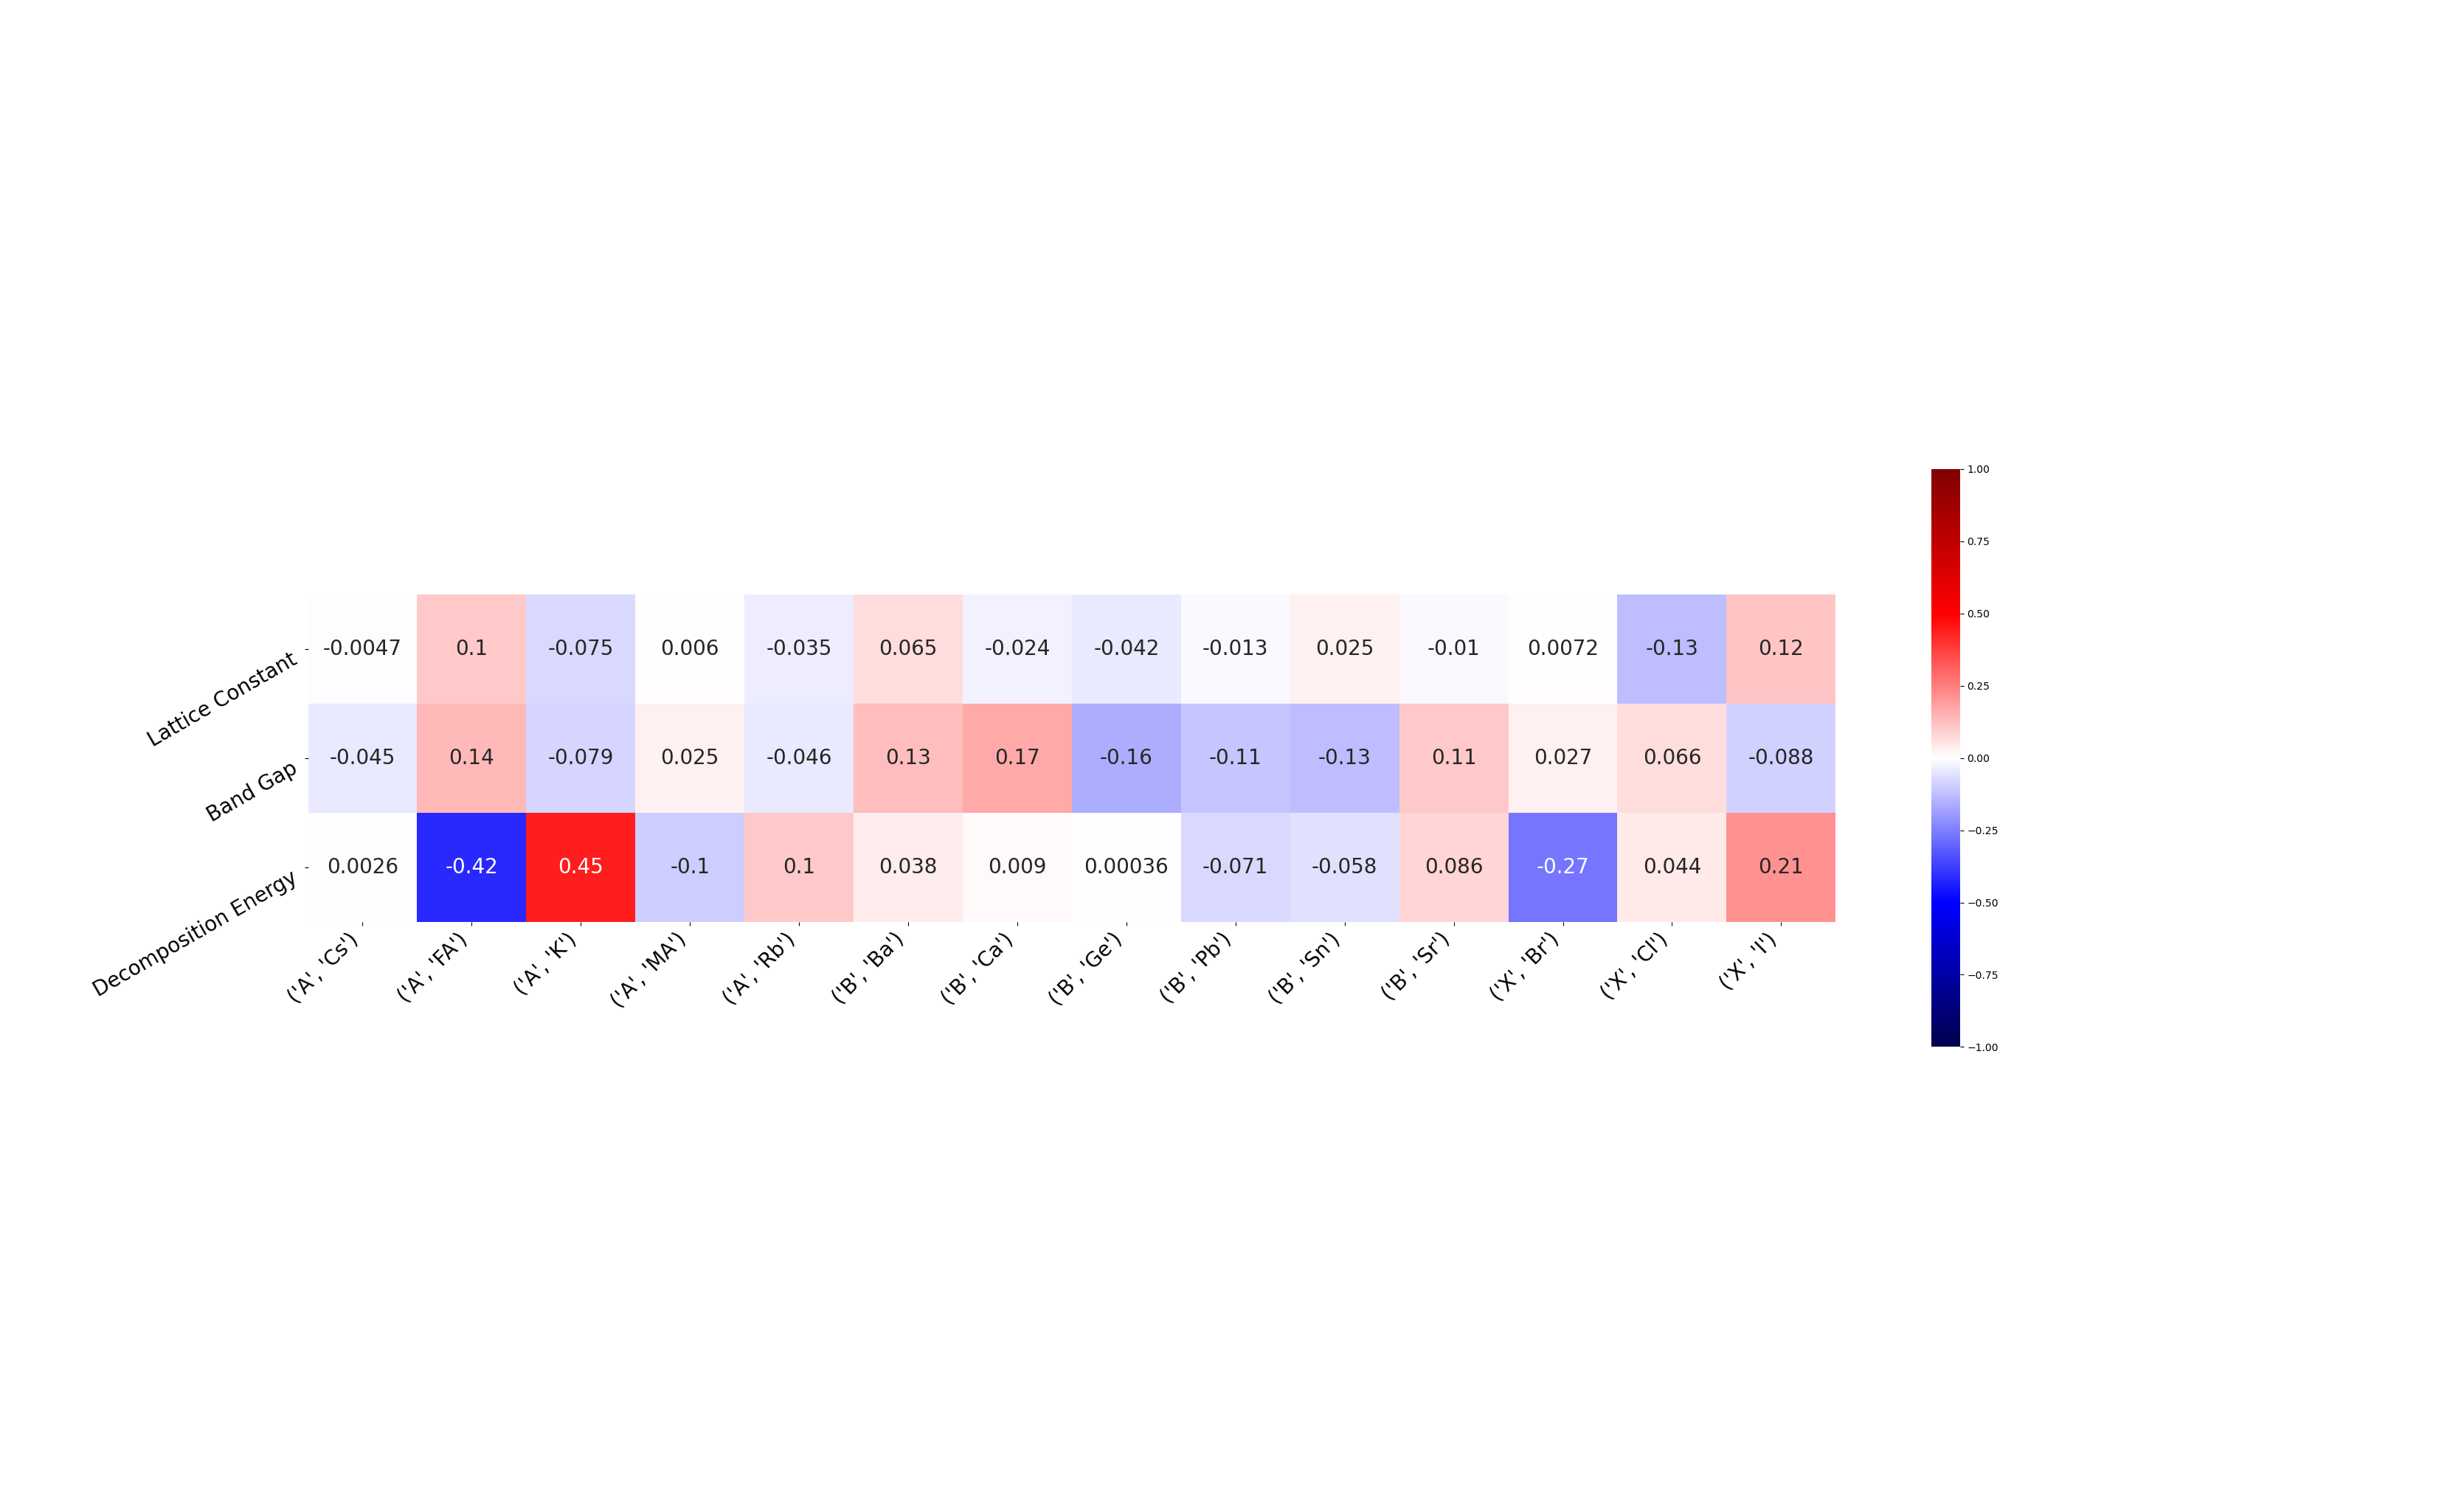
\includegraphics[width=.9\linewidth]{HSE_v_comp_pearson2.png}
\caption{\label{fig:pearson_hcomp} Pearson linear correlation coefficients between 14 composition variables, and 4 HSE computed properties}
\end{figure*}

\begin{figure*}
\centering
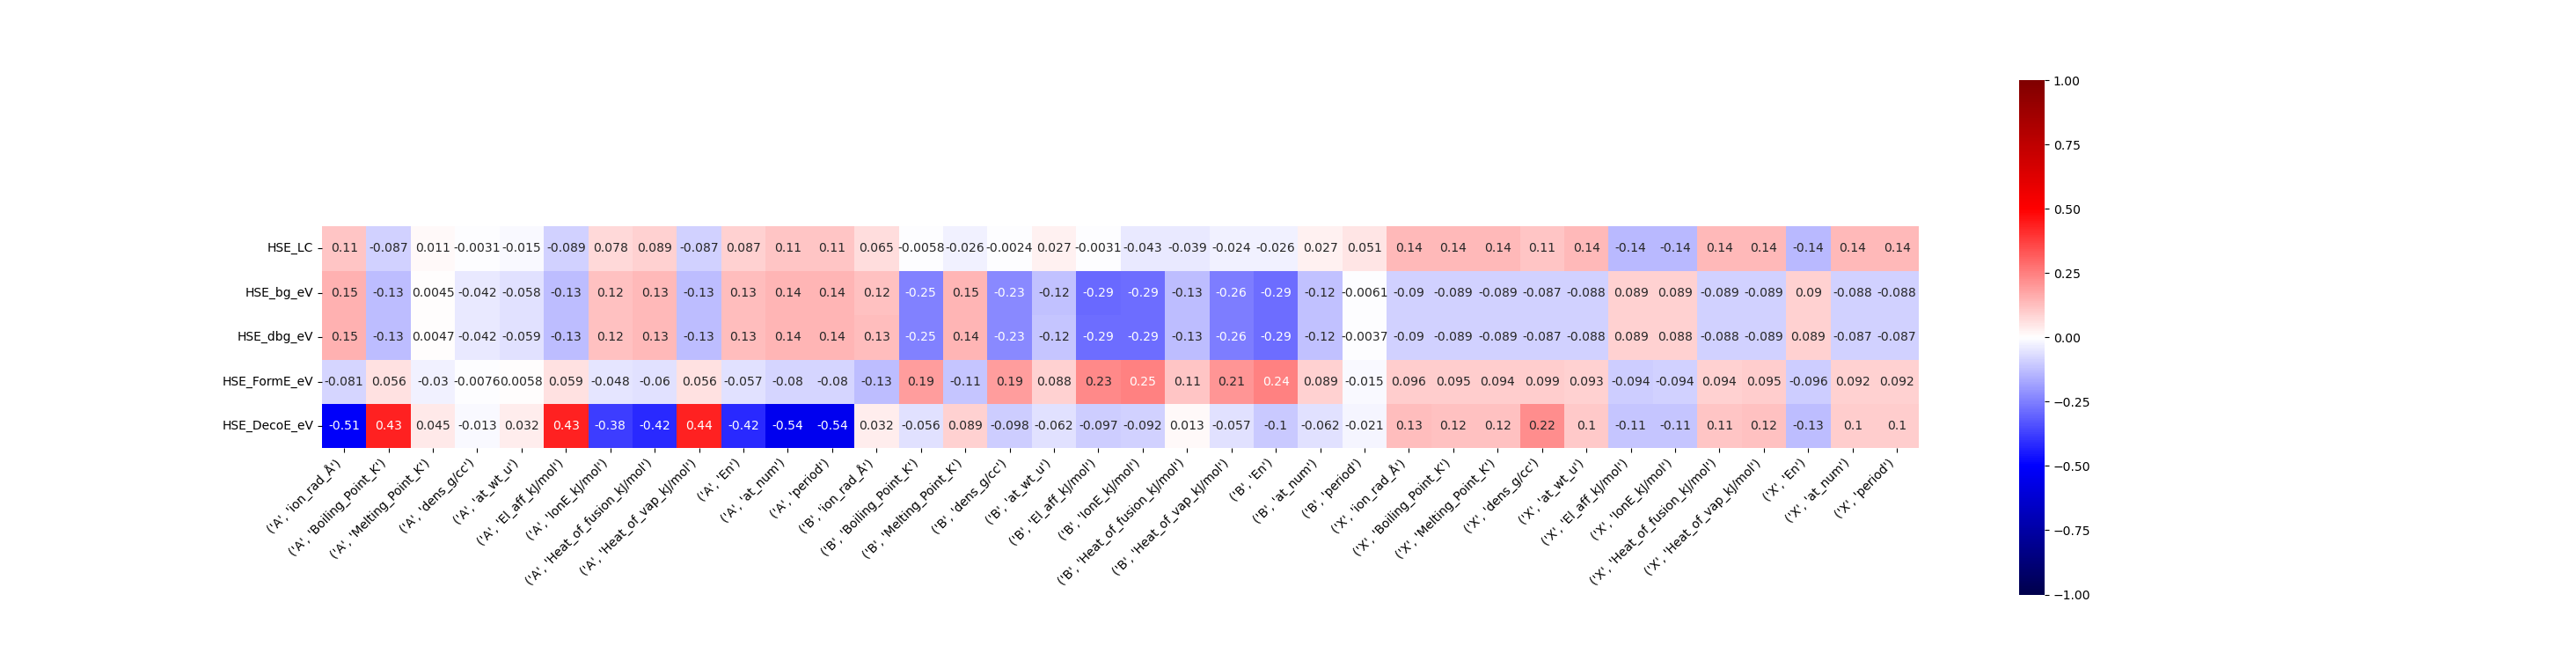
\includegraphics[width=.9\linewidth]{HSE_v_site_prop_pearson.png}
\caption{\label{fig:pearson_hsite} Pearson linear correlation coefficients between 36 composition variables, and 4 HSE computed properties}
\end{figure*}

\begin{figure*}
\centering
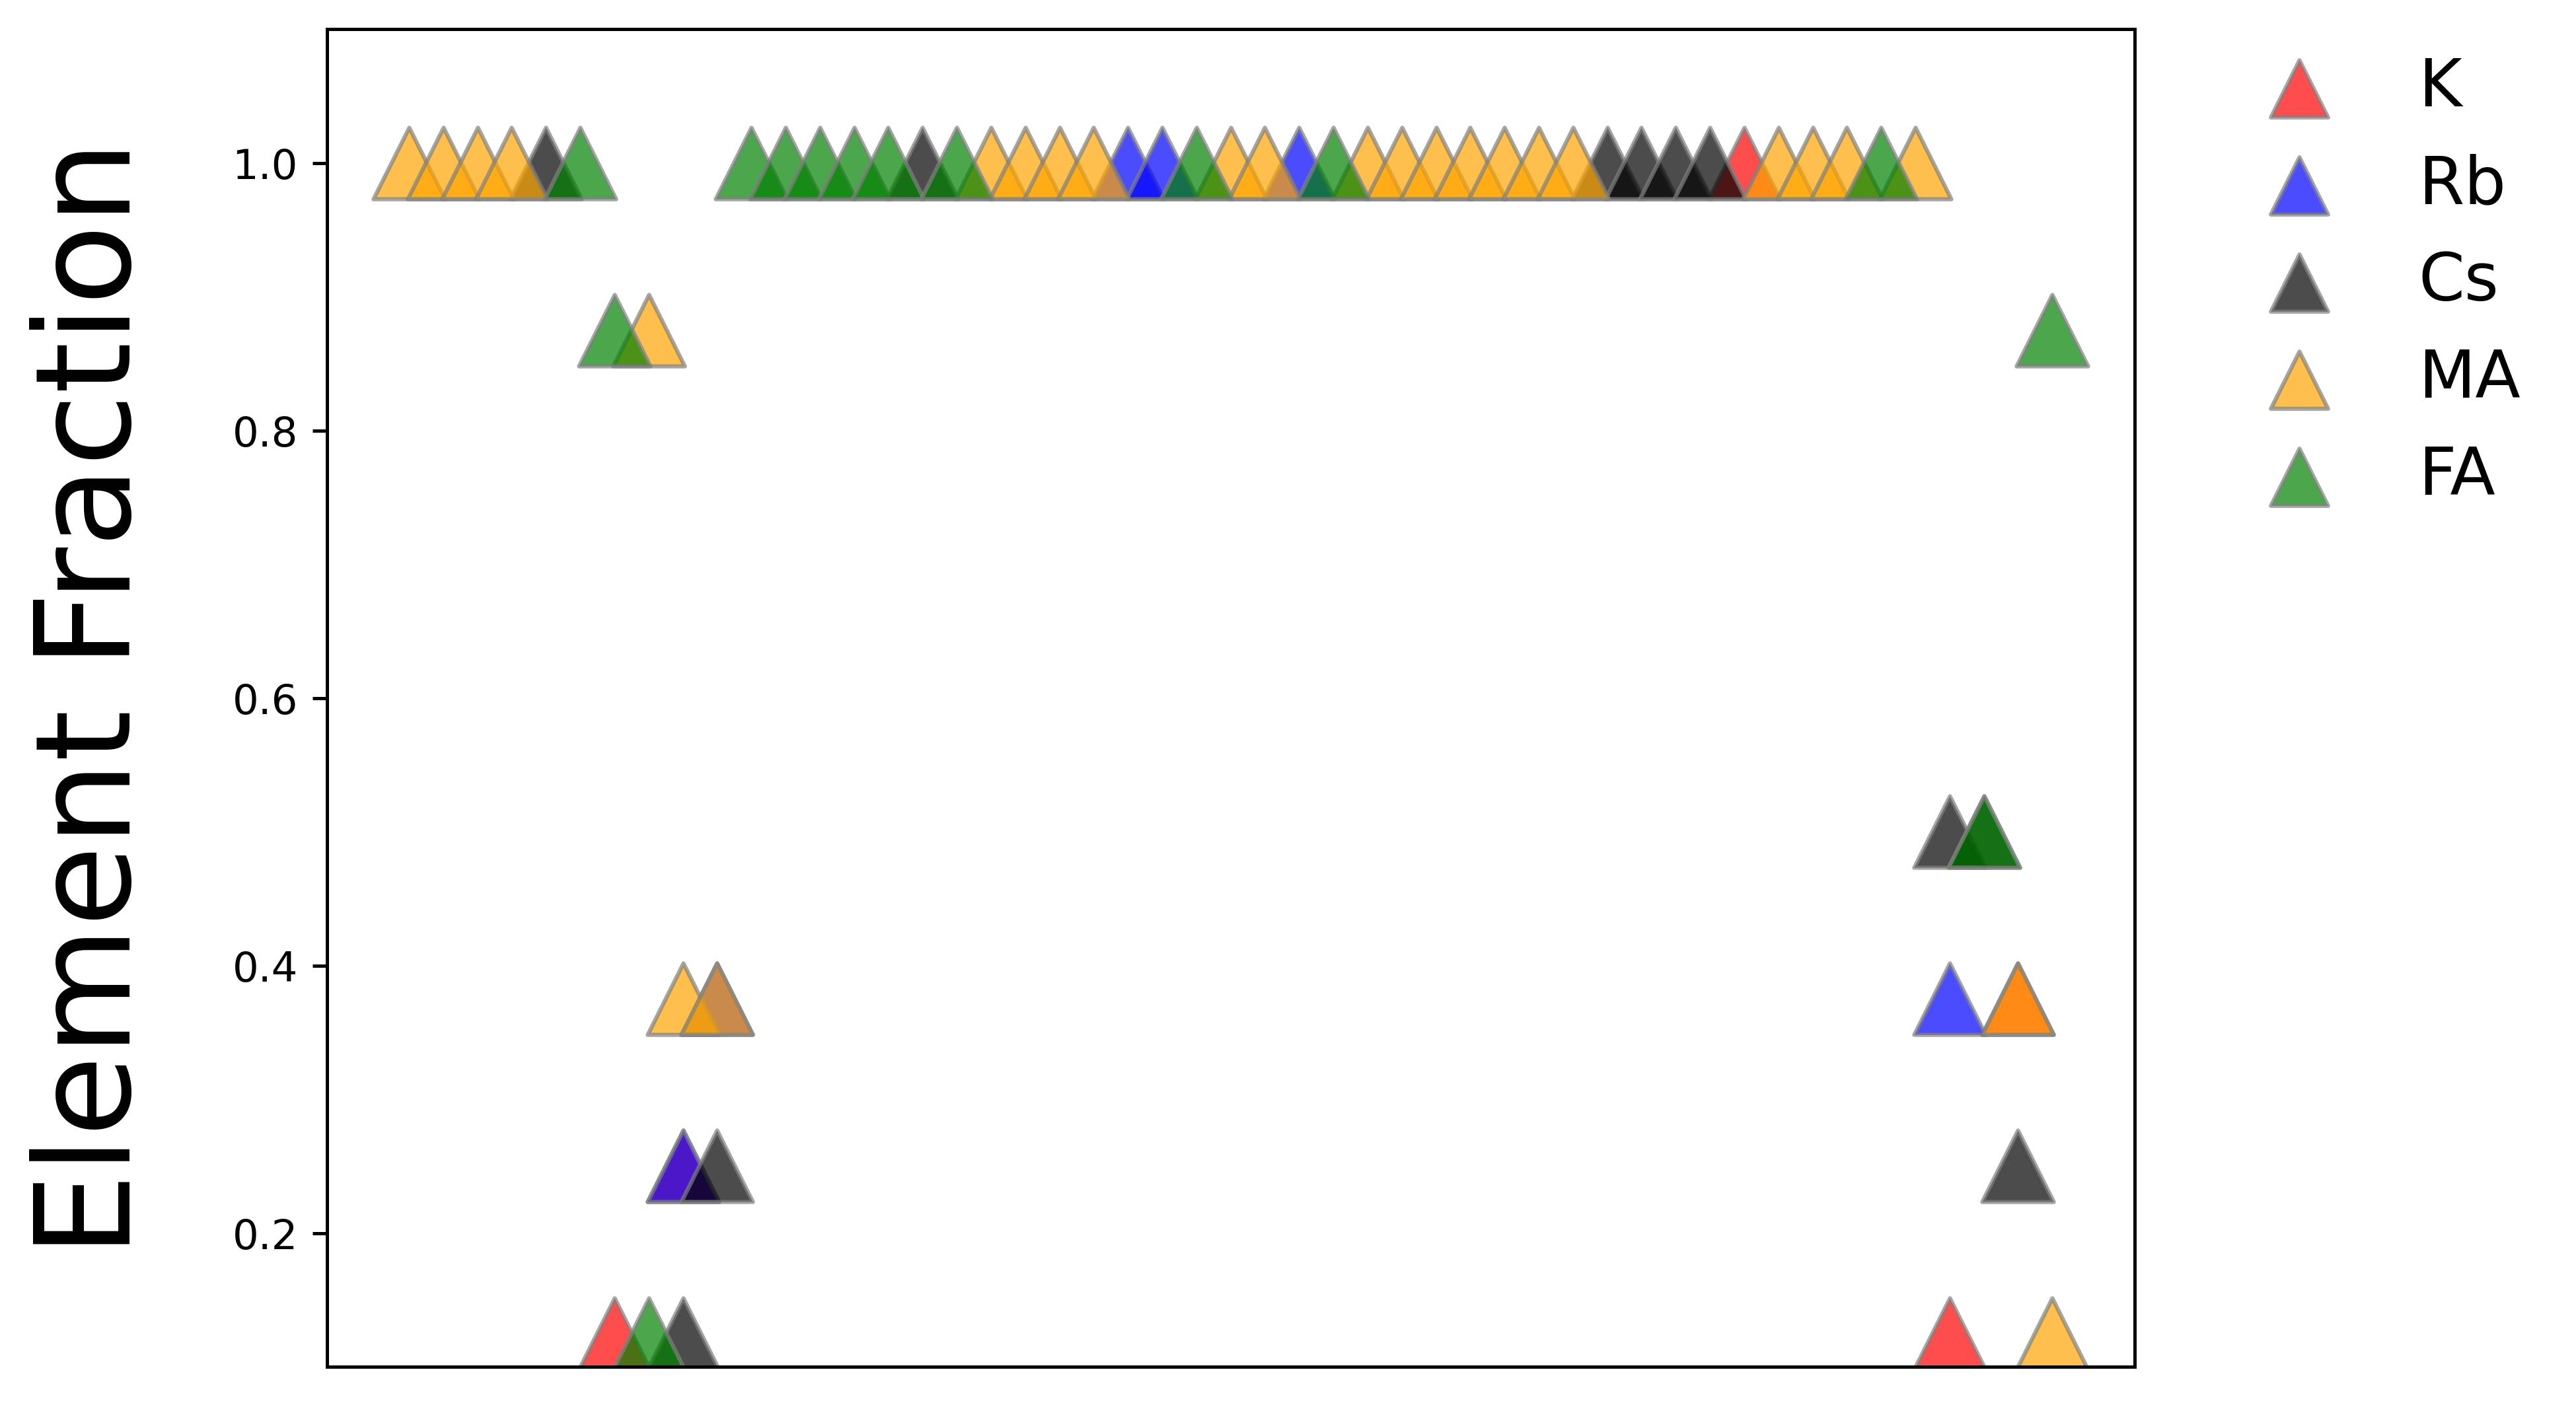
\includegraphics[width=.9\linewidth]{Element_AFrac.jpg}
\caption{\label{fig:sreened_frac_A} Element Fraction for A site elements among all screened perovskites}
\end{figure*}

\begin{figure*}
\centering
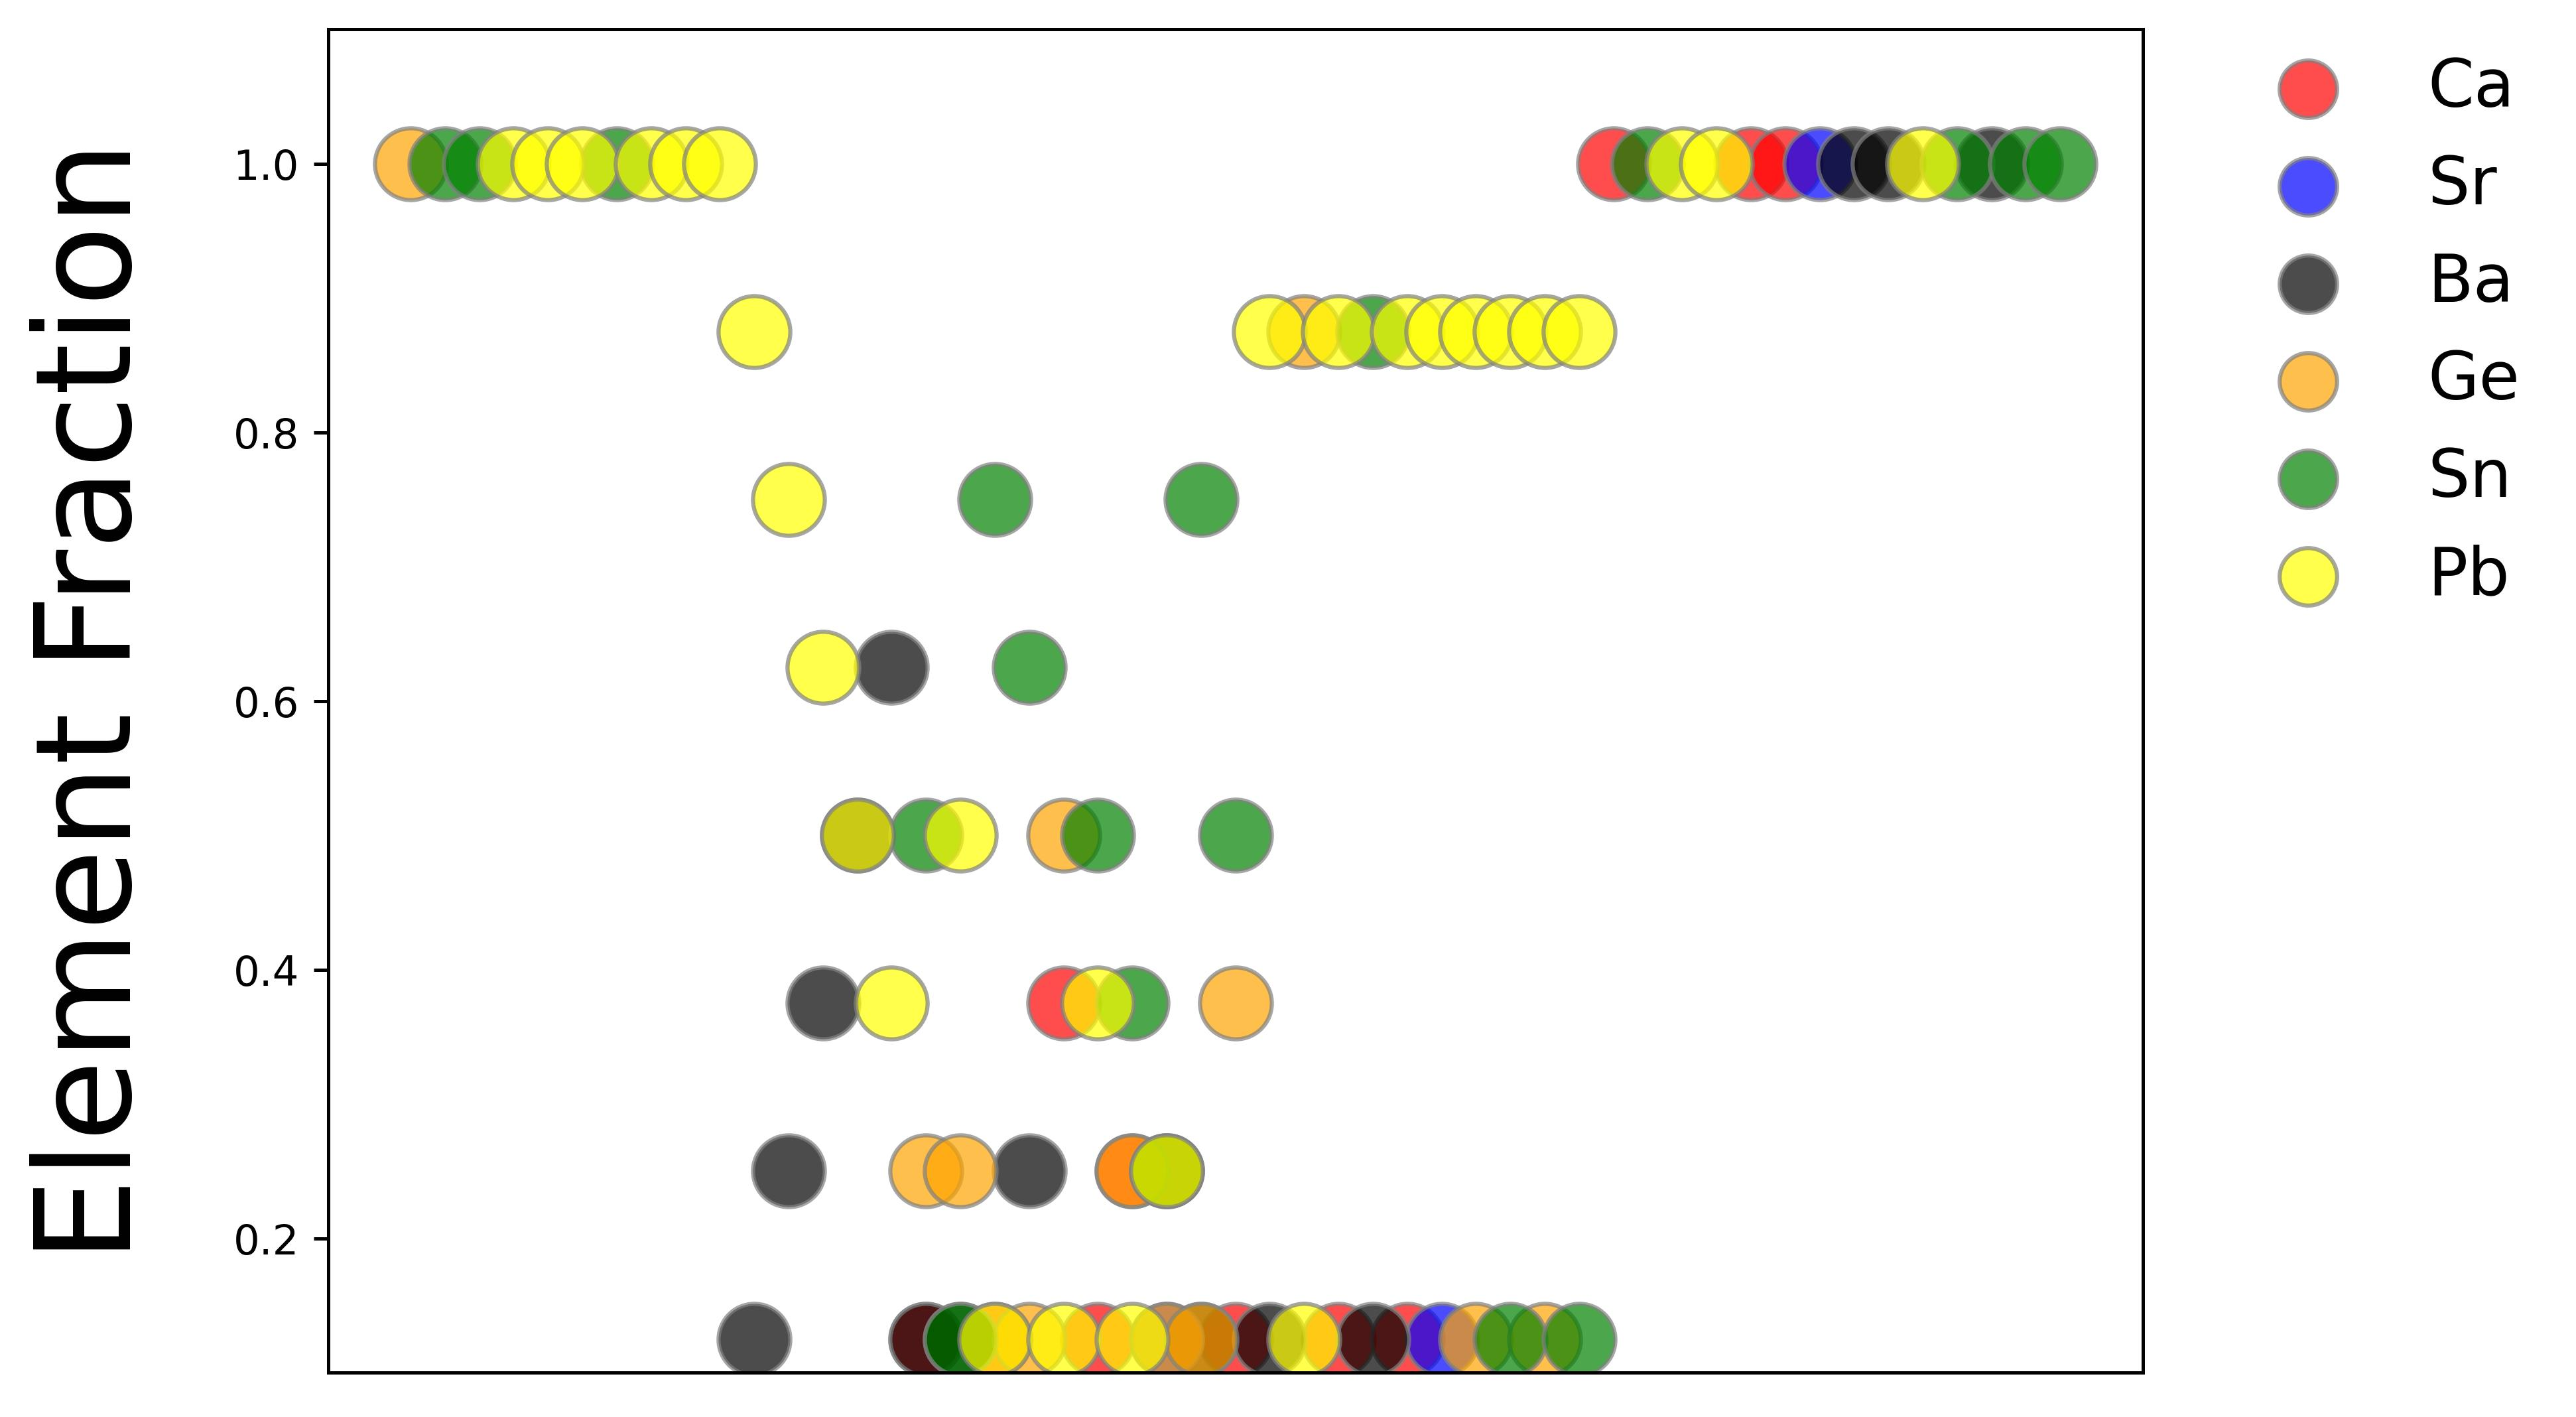
\includegraphics[width=.9\linewidth]{Element_BFrac.jpg}
\caption{\label{fig:sreened_frac_B} Element Fraction for B site elements among all screened perovskites}
\end{figure*}

\begin{figure*}
\centering
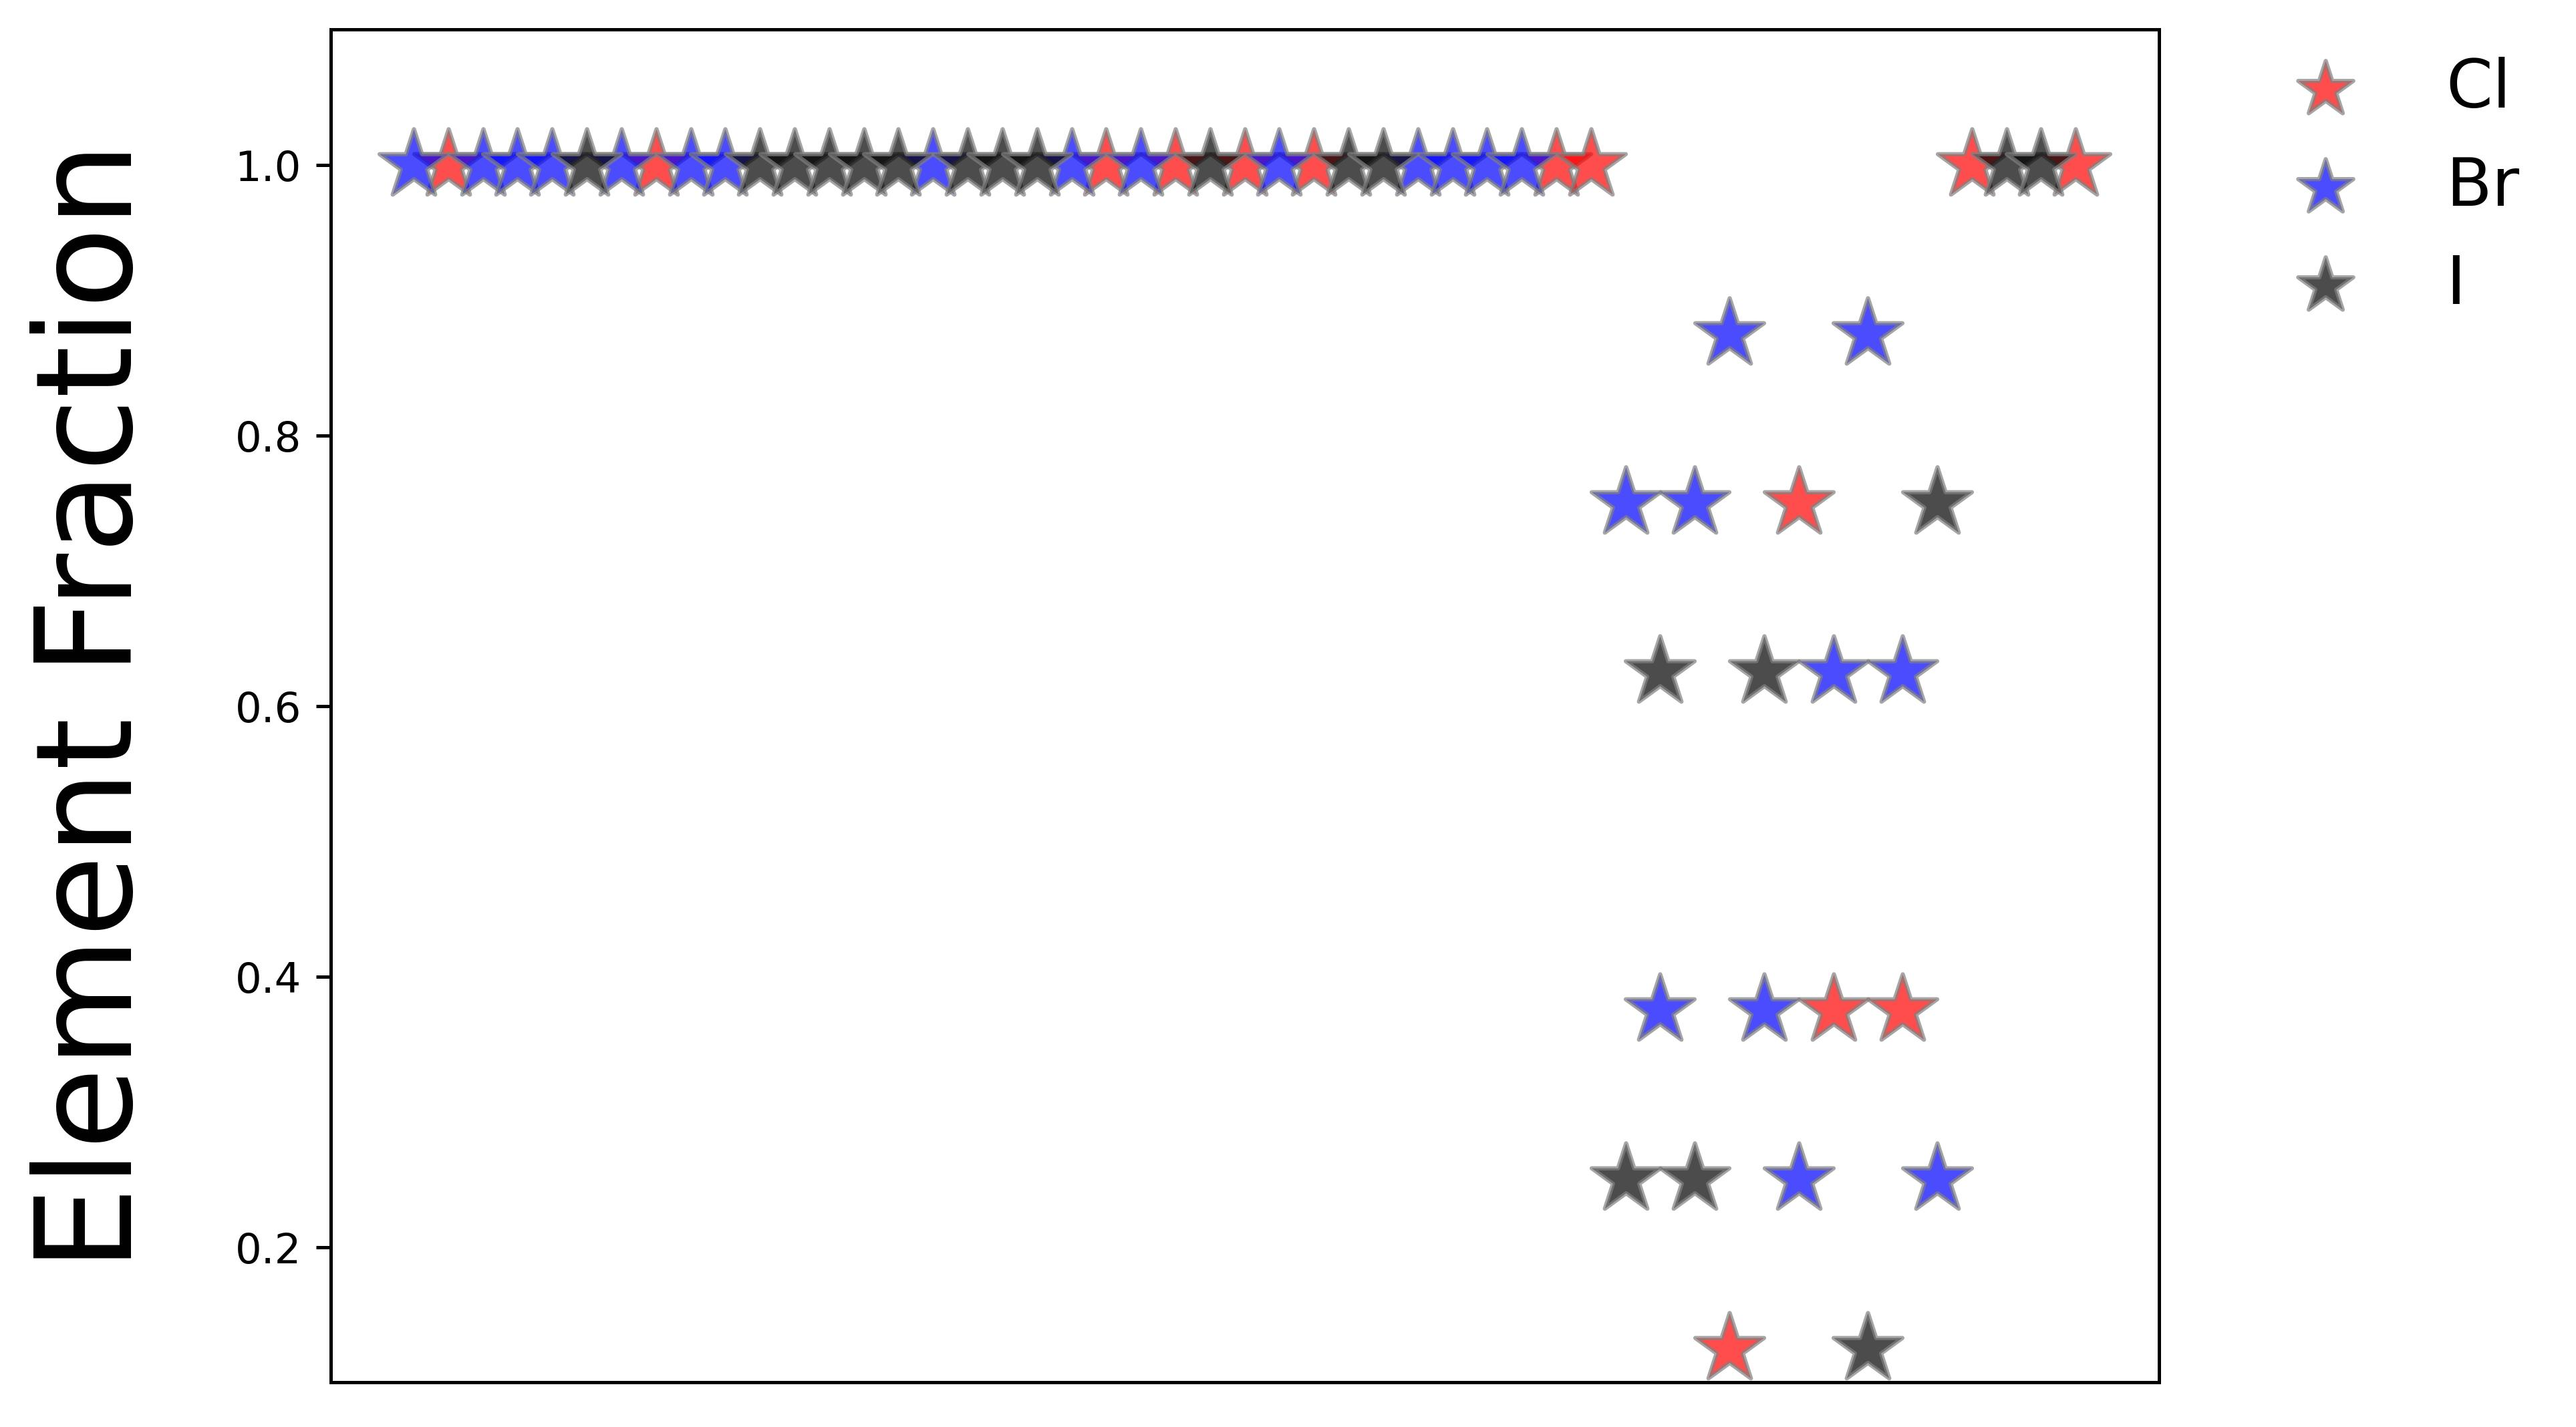
\includegraphics[width=.9\linewidth]{Element_XFrac.jpg}
\caption{\label{fig:sreened_frac_X} Element Fraction for X site elements among all screened perovskites}
\end{figure*}
\end{document}